%% LyX 2.1.4 created this file.  For more info, see http://www.lyx.org/.
%% Do not edit unless you really know what you are doing.
\documentclass[american,fontsize=11pt,paper=a4,twoside,openright,titlepage,numbers=noenddot,headinclude,BCOR=5mm,footinclude=true,cleardoublepage=empty]{scrreprt}
\usepackage[T1]{fontenc}
\setcounter{secnumdepth}{2}
\usepackage{array}
\usepackage{verbatim}
\usepackage{refstyle}
\usepackage{float}
\usepackage{mathrsfs}
\usepackage{mathtools}
\usepackage{multirow}
\usepackage{amsmath}
\usepackage{amsthm}
\usepackage{amssymb}
\usepackage{graphicx}
\usepackage[numbers]{natbib}

\makeatletter

%%%%%%%%%%%%%%%%%%%%%%%%%%%%%% LyX specific LaTeX commands.

\AtBeginDocument{\providecommand\figref[1]{\ref{fig:#1}}}
\AtBeginDocument{\providecommand\chapref[1]{\ref{chap:#1}}}
\AtBeginDocument{\providecommand\propref[1]{\ref{prop:#1}}}
\AtBeginDocument{\providecommand\algoref[1]{\ref{algo:#1}}}
\AtBeginDocument{\providecommand\thmref[1]{\ref{thm:#1}}}
\AtBeginDocument{\providecommand\eqref[1]{\ref{eq:#1}}}
\AtBeginDocument{\providecommand\lemref[1]{\ref{lem:#1}}}
\AtBeginDocument{\providecommand\tabref[1]{\ref{tab:#1}}}
\newcommand{\noun}[1]{\textsc{#1}}
%% Because html converters don't know tabularnewline
\providecommand{\tabularnewline}{\\}
\floatstyle{ruled}
\newfloat{algorithm}{tbp}{loa}[chapter]
\providecommand{\algorithmname}{Algorithm}
\floatname{algorithm}{\protect\algorithmname}
\RS@ifundefined{subref}
  {\def\RSsubtxt{section~}\newref{sub}{name = \RSsubtxt}}
  {}
\RS@ifundefined{thmref}
  {\def\RSthmtxt{theorem~}\newref{thm}{name = \RSthmtxt}}
  {}
\RS@ifundefined{lemref}
  {\def\RSlemtxt{lemma~}\newref{lem}{name = \RSlemtxt}}
  {}


%%%%%%%%%%%%%%%%%%%%%%%%%%%%%% Textclass specific LaTeX commands.
% Classic Thesis Style loader
\makeatother
\input{classicthesis-config.tex}
\makeatletter
% use Latin Modern instead of Computer Modern sans serif
\renewcommand{\sfdefault}{lmss}
\theoremstyle{plain}
\ifx\thechapter\undefined
\newtheorem{thm}{\protect\theoremname}
\else
\newtheorem{thm}{\protect\theoremname}[chapter]
\fi
  \theoremstyle{definition}
  \newtheorem{defn}[thm]{\protect\definitionname}
  \theoremstyle{plain}
  \newtheorem{prop}[thm]{\protect\propositionname}
  \theoremstyle{remark}
  \newtheorem{rem}[thm]{\protect\remarkname}
  \theoremstyle{plain}
  \newtheorem{lem}[thm]{\protect\lemmaname}

%%%%%%%%%%%%%%%%%%%%%%%%%%%%%% User specified LaTeX commands.
\usepackage{algorithm,algpseudocode}
\newref{prop}{name=Proposition~,Name=Proposition~}
\newref{prob}{name=Problem~,Name=Problem~}
\newref{thm}{name=Theorem~,Name=Theorem~}
\newref{chap}{name=Chapter~,Name=Chapter~}
\newref{part}{name=Part~,Name=Part~}
\newref{tab}{name=Table~,Name=Table~}
\newref{algo}{name=Algorithm~,Name=Algorithm~}
\newref{lem}{name=Lemma~,Name=Lemma~}
\newref{fig}{name=Figure~,Name=Figure~}
\newref{chap}{name=Chapter~,Name=Chapter~}
\newref{rem}{name=Remark~,Name=Remark~}
\usepackage{array}
\usepackage{booktabs}
\usepackage[labelfont=bf]{caption}
\MakeRobust{\Call}
\renewcommand{\floatpagefraction}{.9}%

\makeatletter
\renewcommand*{\thetable}{\arabic{chapter}.\arabic{table}}
\renewcommand*{\thefigure}{\arabic{chapter}.\arabic{figure}}
\let\c@table\c@figure
\makeatother 

\areaset[current]{\dimexpr\textwidth+\marginparwidth+\marginparsep}{\textheight}
\setlength{\marginparwidth}{-3.3em}
\setlength{\marginparsep}{-3.3em}

\makeatother

\usepackage{babel}
  \providecommand{\definitionname}{Definition}
  \providecommand{\lemmaname}{Lemma}
  \providecommand{\propositionname}{Proposition}
  \providecommand{\remarkname}{Remark}
\providecommand{\theoremname}{Theorem}

\begin{document}
\frenchspacing
\raggedbottom
\pagenumbering{roman}
\pagestyle{plain}

\begin{comment}
\include{Dedication}

\cleardoublepage{}
\end{comment}


\begin{titlepage}
\begin{addmargin}[-10mm]{-30mm}  %%%%% symmetrical margins
\large
\hfill

\vfill{}


\begin{center}
\begingroup \color{Maroon} \spacedallcaps{\myTitle} \endgroup\\
\bigskip{}
\spacedlowsmallcaps{\mySubtitle}\\
\vfill{}

\par\end{center}

\begin{center}
\medskip{}

\par\end{center}

\begin{center}
\myName
\par\end{center}

\medskip{}


\begin{center}
%\myDepartment\\
%\myFaculty\\
\myUni\\
\myTime
\par\end{center}

\vfill{}


\end{addmargin} 
\end{titlepage} 


\cleardoublepage{}\begingroup
\let\clearpage\relax
\let\cleardoublepage\relax 


\chapter*{Acknowledgments}

I would like to begin by thanking my advisor Neil Shephard not only
for his support throughout the process of writing this thesis, but
also for the tremendous impact he has had on me during my undergraduate
career at Harvard. Neil's teaching over the years inspired in me a
deep interest in the relationship between statistics, mathematics,
and economics; the influence of the ideas he exposed me to on my personal
and intellectual growth could hardly be overstated.

I would also like to thank to Natesh Pillai for several helpful discussions
related to this thesis. In addition, I would like to thank my mentors
at the various firms I have worked at over my summers for making tangible
the links between what I was learning in school and the world as it
really is. I am also indebted to Scott Kominers, who showed me what
great research looks like, and gave me an opportunity to feel just
how exhilarating it could be to wrangle with ideas that I was truly
excited about.

I would further like to acknowledge the Odyssey cluster supported
by the Research Computing Group in the FAS Division of Science at
Harvard University, and the Research Computing Environment supported
by the Institute for Quantitative Social Science at Harvard University,
on which the computations in this thesis were performed.

Next, I would like to thank my blockmates Ramon Galvan and Anita Lo
for being the best of friends since our very first day at Harvard.
Our countless conversations in our dining hall have had and continue
to have a profound impact on how I see the world. I would also like
to thank Spencer Kwon, who inspired me in my sophomore year to push
into academic territory I never thought I would reach, and James Ho,
my fellow adventurer from the top of Mount Baker, along the Dotonbori
canal, to the bottom of the Florida Bay. And of course, I would like
to thank Alice Zhao, without whom I may have never returned to the
second lecture of the class that began my journey to this thesis,
and without whom the second half of college would have been a very
different two years indeed.

Finally, I would like to sincerely thank my parents for always doing
everything in their power to allow me to explore my interests without
limit. The absolutely caring and nurturing environment they created
is the major reason that I and my little brother are where we are
today, and I hope it will also be what leads Jack, if he chooses,
to one day write a thesis that far surpasses this one. 

\endgroup
\cleardoublepage{}\pagestyle{scrheadings}


\chapter*{Abstract}

This thesis investigates a novel and natural generalization of the
theory of maximum likelihood estimation over discretely observed data
from continuous-time stochastic processes. We propose a Kullback-Liebler
divergence minimizing estimator for inference when given distributional
data i.e. when given the distribution of, as opposed to observations
of, a diffusion process at discrete points in time. Examples of such
data include the probabilistic forecasts frequently made in macroeconomics
or meteorology; to the best of our knowledge, we are the first to
propose inferential techniques on stochastic processes when given
data of this sort. We characterize the proposed estimator and develop
a Monte Carlo expectation-maximization algorithm which converges to
the associated estimate. We also develop the first approximate and
exact samplers for a class of generalized diffusion bridges. These
samplers are not only of independent interest, but also necessary
for implementing the simulation-based expectation-maximization algorithm.

Empirically, we confirm the correctness of the proposed methods through
simulation and demonstrate their robustness to various assumptions
made in their derivation. Then, we synthesize the methods developed
in this thesis to propose a generalized bridge-based imputation scheme
for probabilistic forecasts, and apply this scheme to forecasts of
inflation expectations. We show that generalized bridge-based imputation
produces practically meaningful and statistically significant reductions
in out-of-sample Kullback-Liebler divergence from the true distribution
of forecasts relative to a linear interpolation scheme.


\cleardoublepage{}

\include{Contents}

\cleardoublepage{}

\pagenumbering{arabic}


\chapter{Introduction}

\label{chap:Introduction}


\section{The Oracle at Delphi}

On the eve of the second Persian invasion of Greece in the fifth century
BCE, the Oracle at Delphi prophesized the following to the people
of Sparta \citep{macauley}:

\begingroup     \fontsize{10pt}{12pt}\selectfont
\begin{quotation}
Hear your fate, O dwellers in Sparta of the wide spaces;

Either your glorious city must be sacked by the sons of Perses, 

Or, if it be not so, the whole land of Lacedaemon

Shall mourn the death of a king of the house of Heracles.
\end{quotation}
\endgroup

The Spartans, upon receiving this divination, ought to have understood
that their fortunes would likely deteriorate over the course of the
war, culminating in the loss of either their capital city or their
king (King Leonidas, a descendant of Heracles, and three hundred of
his men were driven to take a legendary last stand at Thermopylae
on the basis of this prophecy). It seems that the people of Sparta
learned something that day about the path of their fortunes over time,
not from the observations of data upon which much of modern statistical
inference is built, but rather from a fundamentally uncertain prognostication\textemdash what
we today might call a probabilistic forecast.

Modern probabilistic oracles, though perhaps less prescient than the
Oracle at Delphi, make forecasts in a great variety of domains. Moreover,
many of the variables over which these probabilistic forecasts are
generated can be modeled as stochastic processes. For example, the
distribution of expectations of professional forecasters for various
macroeconomic indicators over time are regularly reported by central
banks around the world. Meteorologists increasingly offer probabilistic
forecasts of everything from the path of cyclones to future humidity
and temperature levels, and market-determined distributions over the
prices of securities on future dates are implied by the prices of
options which expire on those dates (see \citet[Section II in][]{breeden-litzenberger-1978}).
If these forecasts reflect the truth, we can understand them as data
on the future distribution of a particular stochastic process, or
what we will refer to as distributional data. \figref{dist-data}
presents a intuitive visualization of a distributional datum, where
the value axis might represent any numeric value from the price of
a bond to a humidity reading. It ought to be kept in mind that the
depicted marginal distributions may be linked by some dependence structure
over time.

Some natural questions that can be asked of distributional data include:
\begin{aenumerate}
\item ``If we surveyed a group of economists for only their expectations
of one-year-forward inflation, what could we learn about their expectations
of six-months-forward inflation?'', or
\item ``Given the distribution of temperature in Boston a week from now,
what is the probability that the temperature in Boston tomorrow will
be higher than $15^{\circ}\mbox{C}$?'', or
\item ``How is the market pricing the distribution of a stock price between
dates on which the stock's associated options expire?''.
\end{aenumerate}
Though simple to pose, it is not clear what the mathematically rigorous
answers to general questions like these are.
\begin{figure}
\begin{centering}
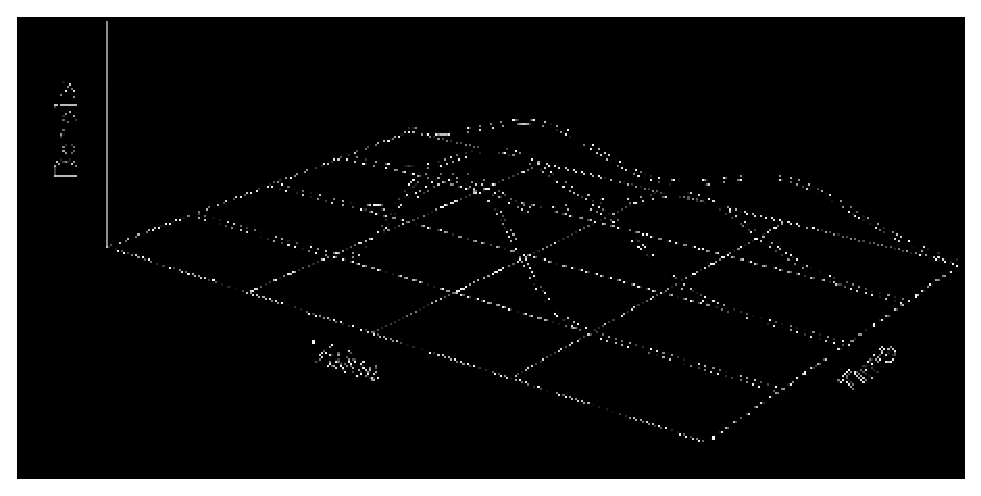
\includegraphics[width=0.5\columnwidth]{/Users/marshall/Documents/senior/thesis/figures/intuition_ed}
\par\end{centering}

\caption{\label{fig:dist-data}An intuitive depiction of a distributional datum.
This particular distributional datum is a four-dimensional joint distribution,
and the four marginal distributions of the data are shown at discrete
points in time.}
\end{figure}


This thesis rather focuses on answering two specific questions that
can be asked of a stochastic process when it is conditioned, in some
sense to be made precise in the next chapter, to follow a given distribution
at discrete future points in time. The first question is one of inference:
\begin{quote}
Can we, given distributional data and a parameterized stochastic process,
learn about the parameters governing the dynamics of the process? 
\end{quote}
The second is one of imputation:
\begin{quote}
Can we, given distributional data and a fully specified stochastic
process, impute the distribution of the process in between the times
at which it is conditioned?
\end{quote}
We will soon see that these questions of inference and imputation
are deeply related, and that the solution to either depends intimately
on the other. The answers to these specific questions allow us to
formulate a well-defined response to the broad questions about inflation,
weather, and stock prices posed above. These sorts of broad questions
abound; by extension, the potential applications of the methods proposed
here are both wide in scope and acute in importance. For instance,
one might imagine that knowing the market-implied distribution of
future stock prices could be immensely valuable. Moreover, references
to inference and imputation on distributional data in the context
of stochastic processes are sparse, if they appear at all, in the
literature. As such, this thesis represents the first investigation,
to the best of our knowledge, into inference on stochastic processes
when they are conditioned to follow a distribution at discrete future
points in time.


\section{Contributions and Related Work}

In the theoretical portion of this thesis, we propose a novel and
natural generalization of the theory of maximum likelihood estimation
over discretely observed data from continuous-time stochastic processes.
This theory begins with \citet{rao-1988} in general and \citet{yoshida-1992}
for the specific case of diffusion processes. In particular, we propose
that it is appropriate to use an estimator that minimizes Kullback-Liebler
(K-L) divergence for inference when given the distribution of a diffusion
process at discrete points in time. This is in contrast to the maximum
likelihood estimator, which is used for inference when given discrete
observations of such a process. We characterize this estimator as
a limiting case of the maximum likelihood estimator, and develop a
novel Monte Carlo expectation-maximization algorithm to conduct minimum
K-L divergence estimation, building on the work of \citet{beskos-2006}. 

However, this only partially answers the question of inference, since
the proposed procedure requires the ability to simulate a particular
generalized notion of a diffusion bridge. We therefore connect the
literature on the simulation of diffusion bridges (see \citet{bladt-sorensen-2014})
with the literature on generalized bridges (see \citet{baudoin-2002})
by proposing approximate and exact simulation strategies for a particular
class of generalized bridges. This answers in full the question of
inference. Simultaneously, we answer the question of imputation, having
gained the ability to draw sample paths of fully specified diffusion
processes whose endpoints are conditioned to follow a given distribution.

In the empirical portion of this thesis, we confirm the correctness
of the exact generalized bridge sampler. We further demonstrate that
the approximate sampler offers samples that are qualitatively similar
to those of the exact sampler at a fraction of the computation cost.
Then, we show empirically that the proposed simulation-based inference
technique on distributional data is unbiased for the K-L divergence
minimizing parameter. Moreover, we show that both the generalized
bridge samplers and the inference technique are robust to various
theoretical assumptions made in their derivations.

Finally, taking theory to practice, we use the proposed inference
scheme to estimate the parameters governing the evolution of inflation
expectations under diffusion models with and without analytically
tractable transition densities. We also propose an imputation scheme
for distributional data under a diffusion model specified only up
to its parameters. To conclude, we show that such a scheme, when applied
to probabilistic forecasts of inflation expectations, reduces the
out-of-sample K-L divergence of imputed distributions from true distributions
in a practically meaningful and statistically significant way relative
to linear interpolation.


\section{Outline}

The next chapter reviews the existing theory of stochastic bridges,
with emphasis on Markov bridges and the generalized bridges of \citet{baudoin-2002}.

With the mathematical underpinnings set, we present the theoretical
portion of this thesis in \chapref{EM} and \chapref{4}. \chapref{EM}
introduces and formalizes the problem of conducting inference on data
in the form of distributions. We propose an estimator for the parameters
governing a diffusion process when given distributional data and offer
interpretations of the resulting estimate in relation to the maximum
likelihood estimate; then, we develop a Monte Carlo expectation-maximization
algorithm which converges to the so-called minimum K-L divergence
estimate. We point out that a sampler for generalized diffusion bridges
is required to implement this algorithm, and in \chapref{4}, we present
approximate and exact versions of such a sampling scheme.

The theory developed in this thesis is applied in \chapref{5} and
\chapref{6}. We conduct a variety of simulations in \chapref{5}
to demonstrate both the correctness and robustness of the proposed
generalized bridge samplers and the Monte Carlo expectation-maximization
algorithm. In \chapref{6}, we synthesize and apply these methods
to model the inflation expectations of professional forecasters.

In \chapref{7}, we conclude and outline future directions for research.



\chapter{Setting the Stage\label{chap:2}}

In this chapter, we describe the setting in which the theoretical
results of this thesis are stated, and review the existing theory
upon which the original results presented in the following chapters
will build.


\section{Objects and Notation}

We first fix the main objects of study and notation. We will work
on the probability space $\left(\Omega,\mathcal{B}\left(\Omega\right),\mathbb{P}\right)$,
where the sample space $\Omega=\mathcal{C}\left(\left[0,1\right],\mathcal{R}\right)$
is the space of real-valued continuous functions $\omega:\left[0,1\right]\rightarrow\mathcal{R}$,
which is equipped with its Borel $\sigma$-algebra $\mathcal{B}(\Omega)$.
As usual, $\Omega$ is endowed with the canonical filtration $\{\mathcal{F}_{t}\}_{t\in[0,1]}$
generated by the canonical process $X=\left\{ X_{t}\right\} _{t\in\left[0,1\right]}$,
defined as 
\[
X_{t}\left(\omega\right)\coloneqq\omega\left(t\right),
\]
where $\omega\in\Omega$. For any subset $\mathcal{T}\subseteq\left[0,1\right]$,
let $X_{\mathcal{T}}=\left\{ X_{t}\right\} _{t\in\mathcal{T}}$ be
the canonical process at times $\mathcal{T}$ and $\mathbb{P}_{\mathcal{T}}$
be the restriction of $\mathbb{P}$ to $\Omega_{\mathcal{T}}\coloneqq X_{\mathcal{T}}(\Omega)$.
In general, we will take the density of a given measure to refer to
its density with respect to the Lebesgue measure unless otherwise
noted.

In the following chapters, we will study in detail time-homogenous
univariate It� diffusions i.e. continuous and strongly Markovian stochastic
processes (see standard references like \citet[Chapter 5 in][]{oksendal}
for details). In particular, we will study processes $X$ of the form
\[
X_{t}=X_{0}+\int_{0}^{t}\mu(X_{s})ds+\int_{0}^{t}\sigma(X_{s})dW_{s},
\]
for a Wiener process $W$ where the second integral is one in the
sense of It�. As per convention, we will refer to such processes as
solutions to the stochastic differential equation (SDE)
\[
dX_{t}=\mu(X_{t})dt+\sigma(X_{t})dW_{t},
\]
with a given initial condition on $X_{0}$. In all diffusions to be
studied, we will assume that $\mu$ and $\sigma$ are suitably regular,
admitting a weakly unique solution (i.e. all solutions have the same
finite-dimensional distributions) and finite speed measure. Note,
for example, that the latter assumption excludes the Wiener process.
Finally, we assume that any diffusion considered satisfies the balance
condition 
\[
p_{t}(x,y)m(x)=p_{t}(y,x)m(y),
\]
where $p_{t}$ and $m$ are the transition density and density of
the speed measure associated with the diffusion. We refer the reader
to \citet[Section 2.1 in][]{bladt-sorensen-2014} for a detailed discussion
of these conditions.

We will denote probability measures by capital letters $\mathbb{P},\mathbb{Q},\dots$
in blackboard boldface. Random variables will be denoted by capital
letters $X,Y,\dots$, and their particular realizations by lower-case
letters $x,y,\dots$ as per convention. Vectors $\mathbf{x},\mathbf{y},\dots,$
will be denoted in boldface. Often, we will suppress set braces in
subscripts i.e. $X_{0,1}$ will denote the value of $X$ at times
$\{0,1\}$, and we will frequently use $\mathbf{x}^{(i)}$ to denote
the $i$th element of a vector of countable length $\mathbf{x}$ to
avoid the overloading of the subscript operator. Having set our notation,
we now review some existing theory related to stochastic bridges which
will form the foundation of the novel theoretical results to be presented
in the following chapters.


\section{Markov and Generalized Bridges}

In this section, we introduce the notion of a Markov bridge, pointing
the reader towards references like \citet[Section 1 in][]{leonard-2014}
for an in-depth exposition of the subject. Then, we will summarize
the relevant results of \citet{baudoin-2002} with respect to generalized
bridge measures, which formalize the notion of conditioning a process
on the distribution of its values. So-called Baudoin conditionings
will feature heavily in the chapters to follow. None of the theory
discussed in this section is original to this thesis.

First, we briefly review the well-known properties of Markov bridges.
Fix $\mathbb{P}$ as a Markov measure. Under fairly general conditions,
like those laid out in \citet[Proposition 4 in][]{fitz-pitman-1993},
$\mathbb{P}$ can be disintegrated as a mixture of regular conditional
measures, 
\[
\mathbb{P}=\int_{\mathcal{R}^{2}}\mathbb{P}(\cdot\mid X_{0}=x,X_{1}=y)\mathbb{P}_{0,1}(dxdy),
\]
where $\mathbb{P}(\cdot\mid X_{0}=x,X_{1}=y)$ exists for all $x,y$
in the state space and can be constructed using Doob's method of $h$-transforms
(see \citet[Section 45 in][]{rogers} for a treatment of Doob's $h$-transform
for continuous-time processes). We refer to such a measure as the
bridge measure $\mathbb{P}^{x,y}$ of $\mathbb{P}$. Note that the
canonical process on $\mathbb{P}^{x,y}$ can be understood as the
canonical process on $\mathbb{P}$, with its endpoints pinned to certain
values at $t=0$ and $t=1$. It can be easily shown that bridge measures
inherit the Markov property i.e. $\mathbb{P}^{x,y}$ is also a Markov
measure. In this thesis, we will focus on measures induced by It�
diffusions, which are a special case of Markov measures; a diffusion
bridge, then, is a diffusion process with its endpoints fixed at certain
values.

The idea of a bridge measure has been expanded upon significantly
in the literature (see, for instance, \citet{alili-2002,baudoin-coutin-2007},
and \citet{sottinen-yazigi-2014}). A generalization of particular
interest to this thesis was first proposed by \citet{baudoin-2002};
rather than conditioning a process on the value of its endpoints,
\citet{baudoin-2002} formalizes the sense in which arbitrary functionals
of a process can be conditioned on their law. We consolidate and present
some of the major results of Baudoin below, working on the usual probability
space $(\Omega,\mathcal{B}(\Omega),\mathbb{P})$. First, we define
a Baudoin conditioning.
\begin{defn}[{\citet[Definition 1 in][]{baudoin-2002}}]
\label{def:conditioning}A Baudoin $(Y,\nu)$-conditioning on the
usual probability space is a tuple $(Y,\nu)$ where 
\begin{aenumerate}
\item $Y$ is an $\mathcal{F}_{1}$-measurable random variable valued in
$\mathcal{R}^{k}$ representing $k$ functionals of the path being
conditioned and
\item $\nu$ is a law representing the conditioning, 
\end{aenumerate}
such that, if the law of $Y$ under $\mathbb{P}$ is $\mathbb{P}_{Y}$,
\begin{aenumerate}
\item $\nu$ is absolutely continuous with respect to $\mathbb{P}_{Y}$
and
\item for $t\in[0,1)$ and $y\in\mathcal{R}^{k}$, there exists a process
$\eta_{t}^{y}$ such that for any $\mathcal{F}_{t}$-measurable and
bounded random variable $Z$, $\mathbb{E}_{\mathbb{P}}\left[Z\mid Y=y\right]=\mathbb{E}_{\mathbb{P}}\left[\eta_{t}^{y}Z\right]$.
\end{aenumerate}
\end{defn}
From this point on, we will always assume that the tuples $(Y,\nu)$
we encounter satisfy the conditions above. The next result demonstrates
the existence and uniqueness of a measure which satisfies intuitive
notions of what it means to be conditioned on the law of a random
variable. Moreover, it says that such a conditioned measure is the
convex diversity minimizing measure with respect to a family of related
probability measures.
\begin{prop}[{\citet[Proposition 3 and 6 in][]{baudoin-2002}}]
\label{prop:pv-1}Fix a Baudoin conditioning $(Y,\nu)$ on the usual
probability space. Then, there exists a unique probability measure
$\mathbb{P}^{\nu}$ such that 
\begin{aenumerate}
\item for any bounded random variable $Z:\Omega\rightarrow\mathcal{R}$,
$\mathbb{E}_{\mathbb{P}^{\nu}}[Z\mid Y]=\mathbb{E}_{\mathbb{P}}[Z\mid Y]$
and
\item the law of $Y$ under $\mathbb{P}^{\nu}$ is $\nu$.
\end{aenumerate}
In particular, for any convex function $\varphi:\mathcal{R}^{+}\rightarrow\mathcal{R}$,
if $\mathbb{E}[|\varphi(d\nu/d\mathbb{P}_{Y})|]$ is bounded, then
$\mathbb{P}^{\nu}$ satisfies
\[
\inf_{\mathbb{Q}\in\mathcal{Q}_{\mathbb{P},\nu,\varphi}}\mathbb{E}_{\mathbb{Q}}\left[\varphi\left(\frac{d\mathbb{Q}}{d\mathbb{P}}\right)\right]=\mathbb{E}_{\mathbb{P}^{\nu}}\left[\varphi\left(\frac{d\mathbb{P}^{\nu}}{d\mathbb{P}}\right)\right],
\]
where $\mathcal{Q}_{\mathbb{P},\nu,\varphi}$ is the set of measures
such that for any $\mathbb{Q}\in\mathcal{Q}_{\mathbb{P},\nu,\varphi}$,
\begin{aenumerate}
\item $\mathbb{Q}$ is absolutely continuous with respect to $\mathbb{P}$,
\item $\mathbb{E}\left[|\varphi\left(d\mathbb{Q}/d\mathbb{P}\right)|\right]$
is bounded, and
\item the law of $Y$ under $\mathbb{Q}$ is $\nu$.
\end{aenumerate}
\end{prop}
We refer to $\mathbb{P}^{\nu}$ as the Baudoin $(Y,\nu)$-conditioning
of $\mathbb{P}$, and the canonical process on $\mathbb{P}^{\nu}$
as the Baudoin $(Y,\nu)$-bridge of the canonical process on $\mathbb{P}$.
\propref{pv-1} is a central result, and shows that of the measures
which are sufficiently similar to $\mathbb{P}$ and under which the
law of $Y$ is $\nu$, the convex diversity minimizing measure is
precisely the measure which coincides with $\mathbb{P}$ on events
independent of $Y$. 

While this characterization is theoretically pleasing, it is not practically
useful in working with $\mathbb{P}^{\nu}$. Fortunately, Baudoin points
out that $\mathbb{P}^{\nu}$ can be disintegrated along the $\sigma$-algebra
generated by $Y$ as
\[
\mathbb{P}^{\nu}=\int_{\mathcal{R}^{k}}\mathbb{P}(\cdot\mid Y=y)\nu(dy),
\]
since the regular conditional probability $\mathbb{P}(\cdot\mid Y=y)$
exists by the existence of $\eta_{t}^{y}$. This observation allows
us to uniquely construct $\mathbb{P}^{\nu}$ when $\eta_{t}^{y}$
exists (which we always assume going forward). In the language of
the discussion regarding Markov bridges above, $\mathbb{P}^{\nu}$
is a mixture of the regular conditional probabilities $\mathbb{P}(\cdot\mid Y=y)$
with respect to some mixing measure $\nu$. Note that by definition,
under $\mathbb{P}^{\nu}$, $Y$ has law $\nu$, and as such $\mathbb{P}^{\nu}=\mathbb{P}$
if and only if $\nu=\mathbb{P}_{Y}$.

With the necessary theoretical foundations set, we move now to the
original portion of this thesis, and formalize the problem of inference
on distributional data.



\chapter{Inference on Distributional Data \label{chap:EM}}

In this chapter, we formalize the problem of inference on distributional
data, and develop a novel Monte Carlo expectation-maximization algorithm
to conduct inference on such data.


\section{Stating and Formalizing the Problem}

We present in this section a generalization, stated informally in
\chapref{Introduction}, of the problem of inference on discretely
observed data from diffusion processes.


\subsection{The Discretely Observed Data Problem}

To begin, we review the problem of inference on diffusion processes
observed at discrete points in time. This is a topic of interest for
many statisticians, in large part due to the prevalence of diffusion
processes in modeling a wide range of phenomena, and the simultaneous
unavailability of continuous observations from such processes in the
real world. Consider a solution to the SDE
\begin{equation}
dX_{t}=\mu_{\theta}(X_{t})dt+\sigma_{\theta}(X_{t})dW_{t},\label{eq:sde-with-theta}
\end{equation}
where $\theta\in\Theta\subseteq\mathcal{R}^{p}$ is an unknown parameter
vector, $W$ is a Wiener process, and $\mu_{\theta}$ and $\sigma_{\theta}$
have known parametric forms up to $\theta$. Let $\mathcal{X}\subseteq\mathcal{R}$
be the state space of $X$. Suppose that we observe fixed values $\bar{\mathbf{x}}=\{\bar{x}_{t_{1}},\dots,\bar{x}_{t_{n}}\}\in\mathcal{X}^{n}$
at a collection of times $\mathcal{T}=\{t_{1}<\cdots<t_{n}=1\}$ where
$t_{1}>0$. Then, the log-likelihood of the data $\bar{\mathbf{x}}$
is 
\[
\ell(\theta\mid\bar{\mathbf{x}})=\sum_{i=1}^{n}\ell_{i}(\theta),
\]
where $\ell_{i}(\theta)=\log p_{\theta,t_{i}-t_{i-1}}(\bar{x}_{t_{i-1}},\bar{x}_{t_{i}})$
and $p_{\theta,t}(x,y)$ is the transition density associated with
(\ref{eq:sde-with-theta}) as usual (we assume $X_{t_{0}}=x_{0}$
is fixed). For many specifications of $\mu_{\theta}$ and $\sigma_{\theta}$,
$p_{\theta,t}(x,y)$ is not analytically tractable, and thus likelihood-based
inference on discretely observed data has historically been understood
to be quite difficult. In particular, maximum likelihood estimation
(MLE) has received significant attention in the literature, with proposed
approaches ranging from \citet{sahalia-2002}'s closed-form analytic
likelihood approximations to the simulation-based strategies of \citet{pedersen-1995}
and \citet{durham-gallant-2002}, and more recently, to imputation-based
techniques advanced by \citet{beskos-2006}. \citet{sorensen-2004}
offers a comprehensive survey of the range of inferential techniques
used for the problem of discretely observed diffusions.


\subsection{From Ex-Post to Ex-Ante}

We now present the central problem of this thesis. We can re-interpret
the discretely observed data problem by supposing we lived at $t_{0}=0$,
and viewing the data $\bar{\mathbf{x}}$ not as values of $X$ that
have already been observed, but rather as values that $X$ will take
on with certainty at future times $\mathcal{T}$ (perhaps as prophesized
by an omniscient Oracle). Modulo philosophical and measure-theoretic
subtleties, the problem has not changed materially: We ought to be
able to conduct likelihood-based inference using $\ell(\theta\mid\bar{\mathbf{x}}),$
so long as it is available, as usual.

This ex-ante perspective allows, however, for the generalization of
interest to this thesis. For we may suppose that instead of knowing
the values of $X$ at times $\mathcal{T}$, we know instead the joint
distribution $\nu$ of these values. Intuitively, knowing $\nu$ ought
to reveal information that we may use to learn about the parameters
governing the dynamics of $X$; on the other hand, the likelihood
function is no longer well-defined, and how to proceed with likelihood-based
inference is therefore unclear. We refer to $\nu$ as distributional
data, in juxtaposition with the observed data that is given in the
context of MLE.

The problems of inference on discretely observed data and on distributional
data are visualized in \figref{mle-intuition}. The fixed data depicted
on the left should help us learn about the dynamics of $X$ through
MLE (for instance, the data looks as if it contains some information
about the drift of $X$). The distributional data on the right, then,
with marginals centered at the fixed data, should contain at least
as much information about the dynamics of $X$, if not more.

\begin{figure}
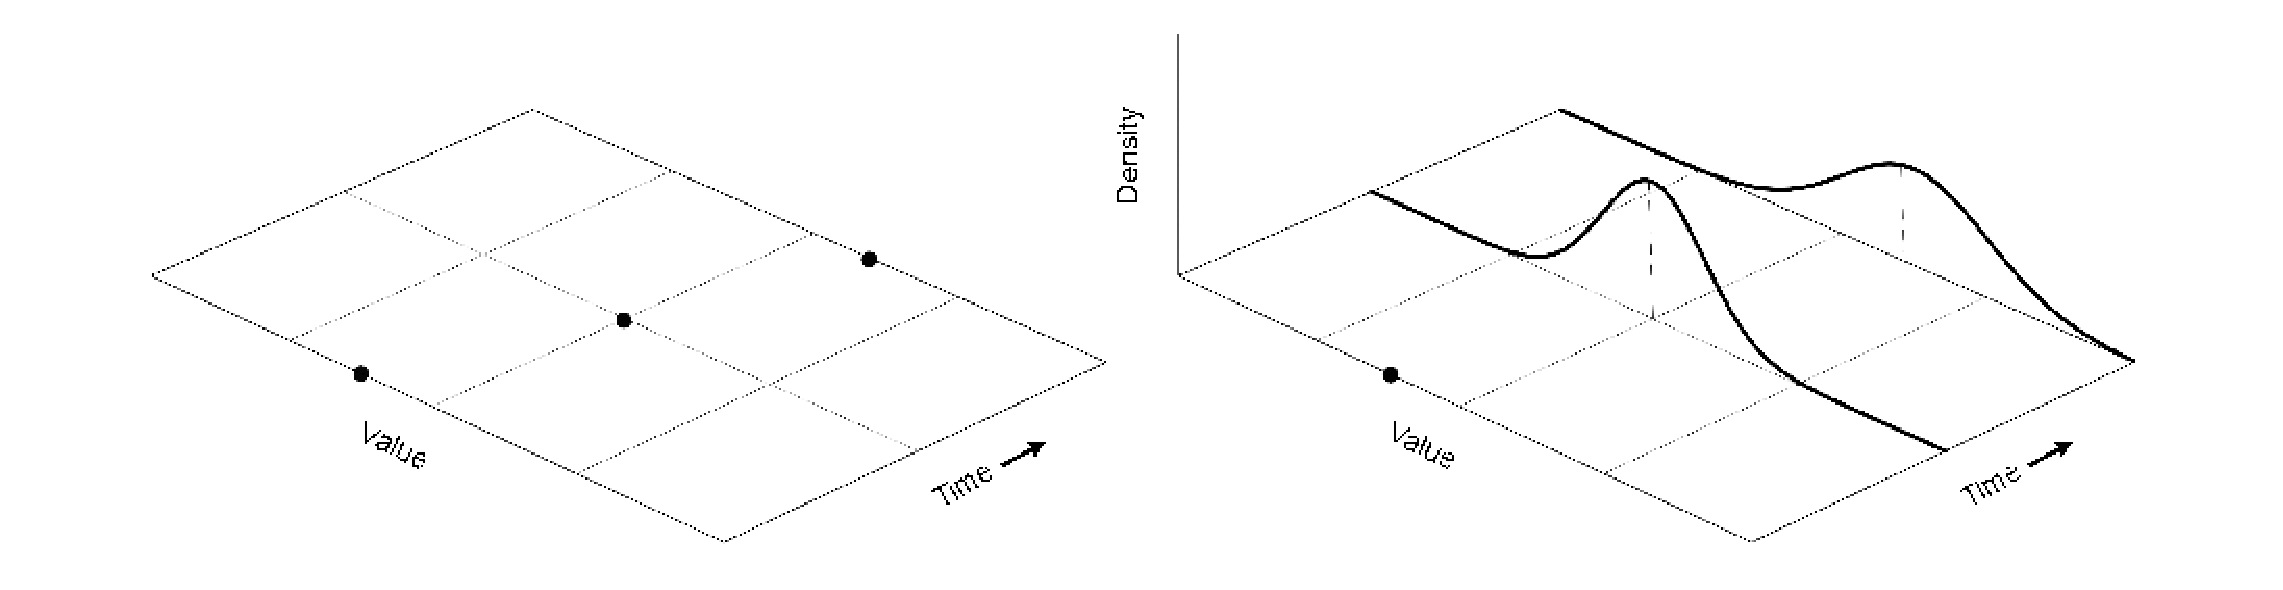
\includegraphics[width=1\columnwidth]{/Users/marshall/Documents/senior/thesis/figures/mle_vs_gen_ed}

\caption{\label{fig:mle-intuition}A visualization of the generalization of
MLE on discretely observed data proposed in this thesis. The value
of the process of interest at $t_{0}$ is fixed and indicated by a
black dot on the value axis. The left graphic depicts a fixed set
of data $\bar{\mathbf{x}}$ over time, on which MLE can be performed
if the log-likelihood is available. The right graphic depicts the
marginal distributions of a set of distributional data, where the
marginal distributions are centered at $\bar{\mathbf{x}}$.}
\end{figure}


In the remainder of this chapter, we will consider the identifiable
family of probability measures $\mathscr{\mathcal{Q}}=\{\mathbb{Q}_{\theta}\mid\theta\in\Theta\}$
on the usual probability space induced by solutions to (\ref{eq:sde-with-theta})
with some fixed initial condition $X_{0}=x_{0}$. We let $\mathbb{Q}_{\theta,X_{\mathcal{T}}}$
be the law of $X_{\mathcal{T}}$ under $\mathbb{Q}_{\theta}$ with
density $Q_{\theta,\mathcal{T}}$, and $\nu$ be an $n$-dimensional
distribution on the usual probability space restricted to times $\mathcal{T}$,
which is absolutely continuous to $\mathbb{Q}_{\theta,X_{\mathcal{T}}}$
for all $\theta\in\Theta$. Then, the problem of inference on distributional
data can loosely be stated as: What, if anything, can we say about
$\theta$, given $X_{\mathcal{T}}\sim\nu$?


\subsection{Proposing and Characterizing an Estimator}

In this subsection, we propose an estimator for $\theta$ given $X_{\mathcal{T}}\sim\nu$,
and make some remarks characterizing its relationship to the maximum
likelihood estimator given discretely observed data.

We first note that from the ex-ante perspective presented above, the
problem of discretely observed data is a special case of the problem
of distributional data. Intuitively, if we were given distributional
data under which $X_{\mathcal{T}}$ was a degenerate random variable,
we would know the values that $X$ would take on with certainty at
future times $\mathcal{T}$ (again, modulo philosophical and measure-theoretic
subtleties). Then, the problem of distributional data could be solved
through traditional MLE. Slightly more formally, we can fix some data
$\bar{\mathbf{x}}\in\mathcal{X}^{n}$. If $\{\nu_{(m)}\}$ is a sequence
of probability measures which are absolutely continuous to $\mathbb{Q}_{\theta,X_{\mathcal{T}}}$
and which converge (in some sense) to the Dirac delta measure $\delta_{\bar{\mathbf{x}}}$,
then as $m\rightarrow\infty$, any estimator for $\theta$ given $X_{\mathcal{T}}\sim\nu_{(m)}$
should coincide with the MLE given $\bar{\mathbf{x}}$. A quantity
that should satisfy this criterion is 
\begin{equation}
\arg\max_{\theta\in\Theta}\int\log Q_{\theta,\mathcal{T}}(x)\nu(dx).\label{eq:mklde}
\end{equation}


We define $\Lambda_{\theta}(\nu)\coloneqq\int\log Q_{\theta,\mathcal{T}}(x)\nu(dx)$,
alluding with our notation to the traditional log-likelihood function
$\ell_{\theta}(\bar{\mathbf{x}})$. We note that $\arg\max_{\theta\in\Theta}\Lambda_{\theta}(\nu)$
is not an estimator in the technical sense since it is a functional
of a distribution $\nu$, rather than a function of observed data.
In this thesis, we will use the term ``estimator'' loosely to refer
to any function(al) of data (distributional or otherwise) that is
used to infer the value of an unknown parameter in a statistical model. 

As \citet[Section 1 in][]{akaike-1973} notes, maximizing $\Lambda_{\theta}(\nu)$
is equivalent to minimizing the K-L divergence of $\mathbb{Q}_{\theta,X_{\mathcal{T}}}$
from $\nu$. This is easily seen by writing 
\begin{eqnarray*}
D(\nu\:||\:\mathbb{Q}_{\theta,X_{\mathcal{T}}}) & = & \mathbb{E}_{\nu}\left[\log\frac{d\nu}{d\mathbb{Q}_{\theta,X_{\mathcal{T}}}}\right]\\
 & = & \mathbb{E}_{\nu}\left[\log\frac{d\nu}{dx}\right]-\mathbb{E}_{\nu}\left[\log\frac{d\mathbb{Q}_{\theta,X_{\mathcal{T}}}}{dx}\right].
\end{eqnarray*}


For this reason, we call the proposed estimator for $\theta$ in (\ref{eq:mklde})
the minimum K-L divergence estimator (MKLDE) given $\nu$. We now
present two remarks, which
\begin{aenumerate}
\item characterize the MKLDE given $\nu$ as a limiting case of maximum
likelihood estimation under model misspecification when $\nu$ is
a true probability model, and
\item show that a (traditional) estimator given finitely many samples from
$\nu$ asymptotically converges to the MKLDE given $\nu$.
\end{aenumerate}
The first remark connects the MKLDE given $\nu$ to the MLE under
model misspecification.
\begin{rem}
\label{rem:misspecification}Let $\nu$ be the true distribution of
$X$ at times $\mathcal{T}$, and consider $N$ i.i.d draws from $\nu$,
$\{X_{\mathcal{T},(i)}\}_{i=1,\dots,N}$. If we wished to model $\nu$
using the family of potentially misspecified probability models $\mathcal{Q}$
restricted to $\mathcal{T}$, the MLE given $\{X_{\mathcal{T},(i)}\}_{i=1,\dots,N}$
would be 
\[
\arg\max_{\theta\in\Theta}\frac{1}{N}\sum_{i=1}^{N}\log Q_{\theta,\mathcal{T}}(X_{\mathcal{T},(i)}).
\]
By a result of \citet[Theorem 2.2 in][]{white-1982}, 
\[
\arg\max_{\theta\in\Theta}\frac{1}{N}\sum_{i=1}^{N}\log Q_{\theta,\mathcal{T}}(X_{\mathcal{T},(i)})\xrightarrow{p}\arg\min_{\theta\in\Theta}\mathbb{E}_{\nu}\left[\log\frac{d\nu}{d\mathbb{Q}_{\theta,X_{\mathcal{T}}}}\right]
\]
as $N\rightarrow\infty$, and thus by the observation of \citet{akaike-1973},
\[
\arg\max_{\theta\in\Theta}\frac{1}{N}\sum_{i=1}^{N}\log Q_{\theta,\mathcal{T}}(X_{\mathcal{T},(i)})\xrightarrow{p}\arg\max_{\theta\in\Theta}\Lambda_{\theta}(\nu),
\]
which is the MKLDE.
\end{rem}
The intuition for this relationship is as follows. Recall that a time-homogenous
Markov measure is uniquely determined by a transition kernel and a
marginal measure; an SDE satisfying the requirements outlined in \chapref{2}
along with the initial condition $X_{0}=x_{0}$ therefore admits a
bijection between $\Theta$ and $\mathcal{Q}$. Now suppose we know
$X_{\mathcal{T}}\sim\nu$. If $\nu$ is not the law of $X_{\mathcal{T}}$
under any element of $\mathcal{Q}$, it must be the case that we have
misspecified our probability model. In this case, the best we can
do is to find the value of $\theta$ that minimizes the K-L divergence
of $\mathbb{Q}_{\theta,X_{\mathcal{T}}}$ from $\nu$, which is precisely
the MKLDE given $\nu$.

In practice, we will often only have access to a finite number of
draws from $\nu$; think, for instance, of the forecasts for humidity
that a panel of finitely many weatherpeople might give. We now remark
on the consistency of the MKLDE given only a fixed number of samples
from $\nu$.
\begin{rem}
\label{rem:bootstrap}Let $\hat{\nu}_{(N)}$ be the empirical distribution
function induced by $N$ draws from $\nu$, and consider $N$ i.i.d
draws from $\hat{\nu}_{(N)}$, $\{X_{\mathcal{T},(i)}\}_{i=1,\dots,N}$.
By standard results demonstrating the consistency of plug-in bootstrap
estimators (see \citet[Section 1 in][]{horowitz-2002}), 
\begin{eqnarray*}
\Lambda_{\theta}(\hat{\nu}_{(N)}) & = & \int\log P_{\theta,\mathcal{T}}(x)\hat{\nu}_{(N)}(dx)\\
 & = & \frac{1}{N}\sum_{i=1}^{N}\log Q_{\theta,\mathcal{T}}(X_{\mathcal{T},(i)})\\
 & \xrightarrow{p} & \Lambda_{\theta}(\nu)
\end{eqnarray*}
and by a loose application of the $\arg\max$ continuous mapping theorem
(see \citet[Theorem 2.7 in][]{kim-pollard-1990}), 
\[
\arg\max_{\theta\in\Theta}\Lambda_{\theta}(\hat{\nu}_{(N)})\xrightarrow{p}\arg\max_{\theta\in\Theta}\Lambda_{\theta}(\nu),
\]
which is the MKLDE given $\nu$.
\end{rem}
This remark shows that an estimator for $\theta$ can be developed
when only given finitely many samples from $\nu$; we simply use the
empirical distribution of the samples as a plug-in estimate for $\nu$
in (\ref{eq:mklde}). This estimator is consistent for the true minimum
K-L divergence parameter, and is an estimator in the traditional technical
sense since $\hat{\nu}$, and by extension $\Lambda_{\theta}(\hat{\nu})$,
is a function of fixed observations. We will simply call this estimator
the MKLDE given $\hat{\nu}$, with the underlying data implicit, in
direct analogy to the MKLDE given $\nu$ defined in (\ref{eq:mklde}),
and refer to both these estimators more generally as the MKLDE.

Together, the two remarks presented above describe why (\ref{eq:mklde})
is statistically meaningful in the context of distributional data.
In particular, suppose $\mathbb{P}$ is a true but unknown probability
model, but the law of $X_{\mathcal{T}}$ under $\mathbb{P}$ is known
to be $\nu$. Then, the MKDLE given $\nu$ over any parameterized
family of probability models $\mathcal{Q}$ identifies the $\mathbb{Q}_{\theta}\in\mathcal{Q}$
such that $\mathbb{Q}_{\theta,X_{\mathcal{T}}}$ has the minimum K-L
divergence from $\nu$. The MKLDE is furthermore asymptotically consistent
when we use the empirical law of samples from $\nu$ as a plug-in
estimate for $\nu$.

While we have shown that the MKDLE is meaningful, given the unavailability
of a transition density for most diffusion processes, it is clear
that $\Lambda_{\theta}(\nu)$ has no obvious functional form for all
but the most specific choices of $\mu_{\theta},\sigma_{\theta}$,
and $\nu$. Solving for the MKLDE is therefore impossible from an
analytic standpoint; the next section addresses this issue by developing
a simulation-based strategy for finding the MKLDE.


\section{Simulation-Based K-L Divergence Minimization}

Simulation-based inference techniques have been applied widely in
the literature to solve the problem of likelihood-based inference
on discretely observed diffusions. This approach began with the seminal
paper of \citet{pedersen-1995}. More recently, \citet{roberts-stramer-2001,elerian-chib-shephard-2001},
and others simultaneously realized that the problem of discrete observations
could be framed in terms of missing data. In particular, though the
likelihood function given discrete observations is in general intractable,
Girsanov's formula can give the likelihood of the observations when
they are augmented with the continuous path of the process in question
between observations. \citet{beskos-2006}, building on techniques
developed by \citet{dempster-1977} and \citet{wei-tanner-1990},
show that the simulation of diffusion bridges (using the Exact Algorithm
of \citet{beskos-roberts-2005}) could be leveraged to supply this
missing data; this approach will be of particular interest to us.

In this section, we generalize the results of \citet{roberts-stramer-2001,beskos-2006},
and \citet{bladt-sorensen-2014} to propose a simulation-based method
to find the MKLDE. As noted above, $\Lambda_{\theta}(\nu)$ cannot
be maximized analytically. However, we use the close parallels between
the MLE given discretely observed data and the MKLDE given distributional
data to develop an MCEM algorithm which converges to $\arg\max_{\theta\in\Theta}\Lambda_{\theta}(\nu)$.


\subsection{The Case of Unit Diffusion Coefficient}

We will first consider the highly specific case of $\sigma_{\theta}(x)$
in (\ref{eq:sde-with-theta}) being equal to unity so that we may
focus deriving the general shape of a simulation strategy. In particular,
we prove the central result of this chapter in this subsection, which
gives a novel EM algorithm which maximizes $\Lambda_{\theta}(\nu)$
in a manner analagous to the EM algorithm of \citet[Section 8 in][]{beskos-2006},
which maximizes $\ell_{\theta}(\bar{\mathbf{x}})$ for discretely
observed data $\bar{\mathbf{x}}\in\mathcal{X}^{n}$.
\begin{thm}
\label{thm:em}Suppose $\sigma_{\theta}(x)=1$ in (\ref{eq:sde-with-theta}).
Then, let $\mathcal{Q}=\{\mathbb{Q}_{\theta}\mid\theta\in\Theta\}$
be the identifiable family of probability measures that are induced
by solutions to (\ref{eq:sde-with-theta}) with constant initial condition.
Fix a parameter estimate $\tilde{\theta}\in\Theta$ and let $\nu$
be a distribution satisfying the usual assumptions. If $\mathbb{Q}_{\tilde{\theta}}^{\nu}$
is the Baudoin $(X_{\mathcal{T}},\nu)$-conditioning of $\mathbb{Q}_{\tilde{\theta}}\in\mathcal{Q}$,
then 
\begin{equation}
\arg\max_{\theta\in\Theta}\Lambda_{\theta}(\nu)-\Lambda_{\tilde{\theta}}(\nu)=\arg\max_{\theta\in\Theta}\mathbb{E}_{\mathbb{Q}_{\tilde{\theta}}^{\nu}}\left[\int_{0}^{1}\mu_{\theta}(X_{s})dX_{s}-\frac{1}{2}\int_{0}^{1}\mu_{\theta}^{2}(X_{s})ds\right].\label{eq:em-equation}
\end{equation}
gives an iteration of an EM algorithm which converges to the MKLDE
given $\nu$. In particular, repeated iterations of (\ref{eq:em-equation})
converge to the parameter $\theta^{*}\in\Theta$ such that the law
of $X_{\mathcal{T}}$ under $\mathbb{Q}_{\theta^{*}}$ has the minimum
K-L divergence from $\nu$, for any $\mathbb{Q}_{\theta}\in\mathcal{Q}$.\end{thm}
\begin{proof}
We begin by re-expressing the objective function on the left hand
side of (\ref{eq:em-equation}) as 
\begin{eqnarray}
\Lambda_{\theta}(\nu)-\Lambda_{\tilde{\theta}}(\nu) & = & \int\log Q_{\theta,\mathcal{T}}(x_{\mathcal{T}})\nu(dx_{\mathcal{T}})-\Lambda_{\tilde{\theta}}(\nu)\nonumber \\
 & = & \int\log\int Q_{\theta,\mathcal{T}}(x_{\mathcal{T}}\mid x)Q_{\theta}(x)dx\nu(dx_{\mathcal{T}})-\Lambda_{\tilde{\theta}}(\nu),\label{eq:firststepem}
\end{eqnarray}
where we take\textbf{ $X$ }to be missing data representing the path
of a solution to (\ref{eq:sde-with-theta}) on $[0,1]$. Then, in
a similar fashion to standard arguments in the derivation of the EM
algorithm (see, for instance, \citet[Section 3.1 in][]{borman-2006}),
we can find from (\ref{eq:firststepem}) that

\begin{align}
\Lambda_{\theta}(\nu)-\Lambda_{\tilde{\theta}}(\nu) & \geq\iint\log\left(\frac{Q_{\theta,\mathcal{T}}(x_{\mathcal{T}}\mid x)Q_{\theta}(x)}{Q_{\tilde{\theta}}(x\mid x_{\mathcal{T}})}\right)P_{\tilde{\theta}}(x\mid x_{\mathcal{T}})dx\nu(dx_{\mathcal{T}})-\Lambda_{\tilde{\theta}}(\nu)\nonumber \\
 & =\iint\log\left(\frac{Q_{\theta,\mathcal{T}}(x_{\mathcal{T}}\mid x)Q_{\theta}(x)}{Q_{\tilde{\theta}}(x\mid x_{\mathcal{T}})Q_{\tilde{\theta},\mathcal{T}}(x_{\mathcal{T}})}\right)P_{\tilde{\theta}}(x\mid x_{\mathcal{T}})dx\nu(dx_{\mathcal{T}}).\label{eq:Deltatn}
\end{align}
We define the quantity in (\ref{eq:Deltatn}) as $\Delta(\theta\mid\tilde{\theta})$,
and let $\mathscr{Q}(\theta\mid\tilde{\theta})\coloneqq\Lambda_{\tilde{\theta}}(\nu)+\Delta(\theta\mid\tilde{\theta})\leq\Lambda_{\theta}(\nu)$.
It can be shown by standard arguments that $\mathscr{Q}(\tilde{\theta}\mid\tilde{\theta})=\Lambda_{\tilde{\theta}}(\nu$),
and so any $\theta$ that increases $\mathscr{Q}(\theta\mid\tilde{\theta})$
must also increase $\Lambda^{\nu}(\theta)$. To maximize this increase,
it suffices to solve for
\begin{eqnarray*}
\arg\max_{\theta\in\Theta}\mathscr{Q}(\theta\mid\tilde{\theta}) & = & \arg\max_{\theta\in\Theta}\iint\log\left(\frac{Q_{\theta,\mathcal{T}}(x_{\mathcal{T}}\mid x)Q_{\theta}(x)}{Q_{\tilde{\theta}}(x\mid x_{\mathcal{T}})Q_{\tilde{\theta},\mathcal{T}}(x_{\mathcal{T}})}\right)Q_{\tilde{\theta}}(x\mid x_{\mathcal{T}})dx\nu(dx_{\mathcal{T}})\\
 & = & \arg\max_{\theta\in\Theta}\iint\log Q_{\theta}(x)Q_{\tilde{\theta}}(x\mid x_{\mathcal{T}})dx\nu(dx_{\mathcal{T}})\\
 & = & \arg\max_{\theta\in\Theta}\int\log Q_{\theta}(x)\mathbb{Q}_{\tilde{\theta}}^{\nu}(dx).
\end{eqnarray*}
The first equality follows from dropping terms that are constant with
respect to $\theta$, including $Q_{\theta,\mathcal{T}}(x_{\mathcal{T}}\mid x)$
since the full path $x$ is fixed. The second equality follows from
the assumption of some regularity conditions that allow for switching
the order of integration and the existence of the requisite densities,
and from the definition of a Baudoin conditioning.

By Girsanov's theorem, since the complete path $X$ has unit diffusion
coefficient, we may write 
\[
\log Q_{\theta}(X)=\int_{0}^{1}\mu_{\theta}(X_{s})dx_{s}-\frac{1}{2}\int_{0}^{1}\mu_{\theta}^{2}(X_{s})ds,
\]
and (\ref{eq:em-equation}) follows. As in any EM algorithm, repeated
iterations of $\tilde{\theta}=\arg\max_{\theta\in\Theta}Q(\theta\mid\tilde{\theta})$
will converge to $\arg\max_{\theta\in\Theta}\Lambda_{\theta}(\nu)$,
which is precisely the MKLDE.
\end{proof}
Note that when $\nu=\delta_{\bar{\mathbf{x}}}$ (in some limiting
sense) for fixed data $\bar{\mathbf{x}}$ observed at $\mathcal{T}$,
(\ref{eq:em-equation}) reduces to 
\[
\arg\max_{\theta\in\Theta}\ell(\theta\mid\bar{\mathbf{x}})-\ell(\tilde{\theta}\mid\bar{\mathbf{x}})=\arg\max_{\theta}\mathbb{E}_{X\mid\bar{\mathbf{x}},\tilde{\theta}}\left[\int_{0}^{1}\mu_{\theta}(X_{s})dX_{s}-\frac{1}{2}\int_{0}^{1}\mu_{\theta}^{2}(X_{s})ds\right]
\]
where the expectation is taken over traditional diffusion bridges
$X$ conditioned on $\bar{\mathbf{x}}$. This equation is simply the
EM algorithm of \citet{beskos-2006} for discretely observed data. 

Though (\ref{eq:em-equation}) is intractable, given the ability to
sample $X$ under $\mathbb{Q}_{\tilde{\theta}}^{\nu}$, it is suggestive
of a Monte Carlo implementation of the EM algorithm following \citet{wei-tanner-1990}.
But before developing such an implementation, we generalize (\ref{eq:em-equation})
for the case of diffusion coefficients known only up to $\theta$.


\subsection{Augmentation Under the Lamperti Transform}

The restriction of the diffusion coefficient to unity severely reduces
the utility of the EM algorithm in practical settings. In this subsection,
we relax this assumption and derive an EM algorithm suitable for general
use. Our general strategy to deal with a diffusion with general diffusion
coefficient is to first transform it into one with unit diffusion
coefficient. Then, after some further transformations, we can derive
the log-likelihood of such a transformed process using Girsanov's
theorem, and substitute this likelihood into (\ref{eq:em-equation}).

Recall that for any solution to (\ref{eq:sde-with-theta}), we may
define the Lamperti transform $\eta_{\theta}(x)$, where
\[
\eta_{\theta}(x)=\int_{x^{*}}^{x}\frac{1}{\sigma_{\theta}(y)}dy,
\]
for appropriate but otherwise arbitrary $x^{*}$. If we set $Y_{t}=\eta_{\theta}(X_{t})$,
by It�'s lemma, $Y$ is the solution to the stochastic differential
equation
\begin{equation}
dY_{t}=\alpha_{\theta}(Y_{t})dt+dW_{t},\label{eq:eta-y}
\end{equation}
where 
\[
\alpha_{\theta}(y)=\frac{\mu_{\theta}(\eta_{\theta}^{-1}(y))}{\sigma_{\theta}(\eta_{\theta}^{-1}(y))}-\frac{1}{2}\sigma_{\theta}^{'}(\eta_{\theta}^{-1}(y)).
\]
We use $\mathbb{Y}_{\theta}$ to denote the measure induced by a solution
to (\ref{eq:eta-y}) with constant initial condition $Y_{0}=\eta_{\theta}(x_{0}).$ 

(\ref{eq:eta-y}) reveals that the Lamperti transform is a continuous
transformation which reduces the diffusion coefficient of any diffusion
to unity. However, \citet{bladt-sorensen-2014} point out that under
the Lamperti transform, the distribution of $Y$ at times $\mathcal{T}$
becomes dependent on the parameter $\theta$, while the EM algorithm
requires that the given data remain fixed with respect to $\theta$.
We adapt their proposed solution to our problem, referring the reader
to \citet[Section 4.1 in][]{bladt-sorensen-2014}, who build on techniques
developed in \citet[Section 3.2 in][]{roberts-stramer-2001} and \citet[Section 8.2 in][]{beskos-2006},
for the theoretical details of the approach. 

Heuristically, our solution is to generate paths of $Y$ under $\tilde{\theta}$
and apply linear transformations to these paths so that they ``look''
like paths under $\theta$. In this way, for each iteration of the
EM algorithm, the given distributional data remains fixed with respect
to $\theta$. In particular, we consider $t_{i-1}\leq t\leq t_{i}$
for each $i=1,\dots,n$. Let $Z(\tilde{\theta})$ be a path under
$\mathbb{Y}_{\tilde{\theta}}^{\nu\circ\eta_{\tilde{\theta}}^{-1}}\eqqcolon\mathbb{Z}_{\tilde{\theta}}$
i.e. a solution to (\ref{eq:eta-y}) conditioned to follow the distribution
$\nu\circ\eta_{\tilde{\theta}}^{-1}$ at times $\mathcal{T}$. Setting
$H_{\tilde{\theta}\rightarrow\theta}=\eta_{\theta}\circ\eta_{\tilde{\theta}}^{-1}$,
we define 
\begin{eqnarray*}
Y_{t}^{*}(\theta,\tilde{\theta}) & = & Z_{t}(\tilde{\theta})+\frac{(t_{i}-t)(H_{\tilde{\theta}\rightarrow\theta}(Z_{t_{i-1}}(\tilde{\theta}))-Z_{t_{i-1}}(\tilde{\theta}))}{t_{i}-t_{i-1}}+\\
 &  & \frac{(t-t_{i-1})(H_{\tilde{\theta}\rightarrow\theta}(Z_{t_{i}}(\tilde{\theta}))-Z_{t_{i}}(\tilde{\theta}))}{t_{i}-t_{i-1}}.
\end{eqnarray*}
Note that $Y_{t_{i-1}}^{*}(\theta,\tilde{\theta})=H_{\tilde{\theta}\rightarrow\theta}(Z_{t_{i-1}}(\tilde{\theta}))$
and $Y_{t_{i}}^{*}(\theta,\tilde{\theta})=H_{\tilde{\theta}\rightarrow\theta}(Z_{t_{i}}(\tilde{\theta}))$;
in this sense, $Y_{\mathcal{T}}^{*}$ ``looks'' like it is distributed
according to $\nu\circ\eta_{\theta}^{-1}$, though it is generated
using a path that is only governed by $\tilde{\theta}$. Now, we let
\begin{aenumerate}
\item $A_{\theta}(u)=\int_{u^{*}}^{u}\alpha_{\theta}$ for suitable but
otherwise arbitrary $u^{*}$, and
\item $\nu_{i,j,\dots}$ be the distribution of the $(i,j,\dots)$-th coordinates
of $\nu$
\end{aenumerate}
and use a result of \citet[Lemma 2 in][]{beskos-2006} to find the
conditional expectation of the continuous log-likelihood function
of $Y_{t}^{*}(\theta,\tilde{\theta})$: 
\begin{eqnarray}
\mathscr{Q}(\theta\mid\tilde{\theta}) & = & \mathbb{E}_{\nu_{n}}\left[A_{\theta}(\eta_{\theta}(X_{t_{n}}))\right]-A_{\theta}(\eta_{\theta}(x_{0}))-\nonumber \\
 &  & \sum_{i=1}^{n}\mathbb{E}_{\nu_{i}}\left[\log(\sigma_{\theta}(X_{t_{i}}))\right]-\nonumber \\
 &  & \frac{1}{2}\sum_{i=1}^{n}\mathbb{E}_{\nu_{i-1,i}}\left[(\eta_{\theta}(X_{t_{i}})-\eta_{\theta}(X_{t_{i-1}}))^{2}/(t_{i}-t_{i-1})\right]-\nonumber \\
 &  & \frac{1}{2}\mathbb{E}_{\mathbb{Z}_{\tilde{\theta}}}\left[\int_{0}^{1}\left(\alpha_{\theta}^{2}+\alpha_{\theta}^{'}\right)\left(Y_{s}^{*}(\theta,\tilde{\theta})\right)ds\right].\label{eq:final-q-1}
\end{eqnarray}


\begin{algorithm}
\caption{MCEM for the MKLDE Given Distributional Data $\nu$}


\begin{algorithmic}[1] 
\Function{$\mathscr{Q}$}{$\theta, \tilde{\theta}, \nu, N, M$}
	\State{$\mathscr{Q} \gets  $\Call{mean}{$A_{\theta}(\eta_{\theta}($\Call{sample}{$\nu, N$}$[,n]))$}}
	\State{$\mathscr{Q} \gets \mathscr{Q} \:-\: $\Call{mean}{$A_{\theta}(\eta_{\theta}($\Call{sample}{$\nu, N$}$[,1]))$}}
	\State{$\mathscr{Q} \gets \mathscr{Q} \:-\: $\Call{sum}{\Call{col-means}{$\log(\sigma_{\theta}($\Call{sample}{$\nu, N$}$)$}}}
	\State{$\mathscr{Q} \gets \mathscr{Q} \:-\: $\Call{sum}{\Call{col-means}{\Call{row-diffs}{$\eta_{\theta}($\Call{sample}{$\nu, N$}$)$}$^2}/$\Call{diff}{$\mathcal{T}$}}}
	\For{$t_i$ in $\mathcal{T}$}
		\State{$S_i \gets 0, \Delta \gets t_i - t_{i-1}, \delta \gets \Delta / M$}
		\For{$N$ iterations}
			\State{\textbf{sample} $t$ from $\{0,\delta,\dots,M\delta\}$}
			\State{$\mathbf{Z} \gets$ \Call{exact baudoin-bridge}{$\alpha_{\tilde{\theta}},1,\nu_{i-1,i} \circ \eta_{\tilde{\theta}}^{-1}, M, \Delta$}}
			\State{$Y^{*}_t \gets \mathbf{Z}_{t} + \Delta^{-1}((t_i - t)(H_{\tilde{\theta} \rightarrow \theta} (\mathbf{Z}_0) - \mathbf{Z}_0) + (t-t_{i-1})(H_{\tilde{\theta}\rightarrow\theta}(\mathbf{Z}_\Delta) - \mathbf{Z}_\Delta))$}
			\State{$S_i \gets S_i + (\alpha_{\theta}^2 + \alpha_{\theta}^{'})(Y^{*}_t)/N$}
		\EndFor
		\State{$\mathscr{Q} \gets Q \:-\:\frac{\Delta}{2}S_i$} 
	\EndFor
	\State \Return{$\mathscr{Q}$}
\EndFunction

\Function{find-mklde}{$\theta_0, \nu, N, M$}
	\State{$\tilde{\theta} \gets \theta_0$}
	\Repeat	
	\State{$\tilde{\theta} = \arg \max_{\theta \in \Theta} \mathscr{Q}(\theta, \tilde{\theta}, \nu, N, M)$}
	\Until{convergence}
	\State \Return{$\tilde{\theta}$}
\EndFunction

\end{algorithmic}

\label{algo:mcem}
\end{algorithm}


Note that by standard Monte Carlo integration results, we may re-write
the last term in (\ref{eq:final-q-1}) as 
\[
\frac{1}{2}\mathbb{E}_{\mathbb{Z}_{\tilde{\theta}},U}\left[\left(\alpha_{\theta}^{2}+\alpha_{\theta}^{'}\right)\left(Y_{U}^{*}(\theta,\tilde{\theta})\right)\right]
\]
for some independent $U\sim\mbox{Unif}[0,1]$. 

While (\ref{eq:final-q-1}) remains hopelessly intractable, it immediately
suggests a MCEM scheme, assuming we have a way of sampling paths under
Baudoin bridge measures. Suppose for the moment we do: the function
\noun{exact baudoin-bridge}(\textbf{\noun{$\mu,\sigma,\nu,M,\Delta$}})
will return discrete observations $\mathbf{X}=\{\mathbf{X}_{t}\}_{t=0,\delta,\dots,M\delta}$
for $\delta=\Delta/M$ of an It� diffusion with drift coefficient
$\mu(x)$ and diffusion coefficient $\sigma(x)$ under the Baudoin
$(X_{0,\Delta},\nu)$-conditioning of its associated measure on $[0,\Delta]$,
where $\Delta\in(0,1]$. Further suppose we have a function \noun{sample($\nu,N$)}
which returns $N$ samples from $\nu$ in a $N\times n$ array. Then,
\algoref{mcem} presents an MCEM algorithm which iteratively maximizes
a Monte Carlo estimate for (\ref{eq:final-q-1}). In particular, the
algorithm converges to the MKLDE, which is the $\theta$ that minimizes
the K-L divergence of the law of $X_{\mathcal{T}}$ under $\mathbb{Q}_{\theta}$
from $\nu$. Note that we exploit the Markovian nature of the measuresin
question to split the evaluation of the last term in (\ref{eq:final-q-1})
into bridges on $[t_{i-1},t_{i}]$ for $i=1,\dots,n$. Furthermore,
we simulate new samples from $\nu$ at every possible point in the
algorithm as a simple method of Monte Carlo variance reduction.

One technical point we must address before continuing is the use of
\algoref{mcem} when only a finite number of samples from $\nu$ is
available i.e. when we wish to use MCEM to find the MKLDE given the
empirical law $\hat{\nu}$ of samples from $\nu$. We note that $\hat{\nu}$
is not absolutely continuous to any measure induced by a solution
to (\ref{eq:sde-with-theta}), and thus a Baudoin $(X_{\mathcal{T}},\hat{\nu})$-conditioning
on such a measure is not well-defined. However, the intuition behind
such a conditioning still holds ($X_{\mathcal{T}}$ is conditioned
to follow a discrete distribution $\hat{\nu}$), and we will demonstrate
in \chapref{5} that using $\hat{\nu}$ as a plug-in estimate for
$\nu$ in \algoref{mcem} produces unbiased estimates for the MKLDE
given $\nu$. As such, we will gloss over the technicality of empirical
distributions not being absolutely continuous to diffusion measures
for the remainder of the thesis.

We have thus partially answered the question of inference on distributional
data. There is, in fact, a meaningful estimate of $\theta$ given
$X_{\mathcal{T}}\sim\nu$: this is precisely the value of $\theta$
which minimizes the K-L divergence of $\mathbb{Q}_{\theta,X_{\mathcal{T}}}$
from $\nu$ when we fix a family of potentially misspecified probability
models $\mathcal{Q}=\{\mathbb{Q}_{\theta}\mid\theta\in\Theta\}$.
\algoref{mcem} finds such a value. However, to implement this MCEM
scheme, we must have a way to sample $Y$ under the Baudoin $(Y_{0,\Delta},\nu\circ\eta_{\tilde{\theta}}^{-1})$-conditioning
of $\mathbb{Y}_{\tilde{\theta}}$. In other words, for known $\tilde{\theta}$,
we must be able to impute the distribution of $Y$ on $(0,\Delta)$
given $Y_{0,\Delta}\sim\nu\circ\eta_{\tilde{\theta}}^{-1}$. We turn
to this question in the following chapter.

\chapter{The Simulation of Generalized Bridges\label{chap:4}}

In this chapter, we develop methods to sample approximate and exact
generalized bridges. 


\section{$\nu-$bridges}

First, we introduce the notion of a $\nu$-bridge. Consider the solution
$X$ to the stochastic differential equation
\begin{equation}
dX_{t}=\mu(X_{t})dt+\sigma(X_{t})dW_{t},\label{eq:basic-sde}
\end{equation}
satisfying the usual assumptions, where $\mu$ and $\sigma$ are fully
specified (this is unlike (\ref{eq:sde-with-theta}) in the previous
chapter, where the drift and diffusion were only known up to some
parameters) and $W$ is a Wiener process. Suppose $X$ induces the
probability measure $\mathbb{Q}$ on the usual probability space,
fix $\mathcal{T}\subseteq[0,1]$ as a set of times, and let $\nu$
be a distribution that is absolutely continuous to the law of $X_{\mathcal{T}}$
under $\mathbb{Q}$. Then, we can understand the Baudoin $(X_{\mathcal{T}},\nu)$-conditioning
of $\mathbb{Q}$ as a generalized diffusion bridge measure, in the
sense that the canonical process on $\mathbb{Q}^{\nu}$ is a regular
diffusion bridge when $\nu$ is the product of Dirac delta measures.\footnote{This statement is more precisely made in some limiting sense, since
the product measure of Dirac delta measures is not absolutely continuous
to $\mathbb{Q}_{\mathcal{T}}$ when $X$ is an It� diffusion. However,
the product measure of Dirac delta measures can be the limit of a
sequence of probability measures which satisfy such a condition.} Since $\mathbb{Q}$ is Markovian, we may, without loss of generality,
set $\mathcal{T}=\{0,1\}$ and restrict our attention to Baudoin conditionings
of the form $(X_{0,1},\nu)$. Then, a $\nu$-bridge of $X$ is defined
as follows.
\begin{defn}
Let $\nu_{0}$ be the marginal distribution of $\nu$ at $t=0$. Then,
let $X$ be a solution to (\ref{eq:basic-sde}) with $X_{0}\sim\nu_{0}$,
and let $\mathbb{Q}$ be the measure it induces. The $\nu-$bridge
of $X$ is the canonical process under the Baudoin $(X_{0,1},\nu)-$conditioning
of $\mathbb{Q}$, denoted $\mathbb{Q}^{\nu}$.
\end{defn}
Baudoin bridges are well-characterized in highly general settings;
we therefore defer to \citet{baudoin-2002} for a theoretical treatment
of their properties. In this chapter, we instead focus on simulating
$\nu$-bridges, motivated by our MCEM scheme's need to sample from
paths under Baudoin bridge measures.


\section{Approximate Simulation of $\nu$-Bridges}

In this section, we propose a sampler of approximate $\nu$-bridges
and make precise the notion of what it means to be an ``approximate''
bridge.

A substantial literature surrounds the simulation of diffusion bridges
since na�ve simulation attempts will have a unacceptably high rejection
probability when attempting to hit the desired endpoint (which, after
all, is a measure zero event). One can imagine that simulating a $\nu-$bridge
should also be non-trivial, since we are not simply conditioning on
the measure zero event of $\left\{ X_{1}=x_{1}\right\} $, but rather
the ``event'' that $X_{0}$ and $X_{1}$ follow some joint distribution.

An overview of the recent literature in simulating traditional diffusion
bridges can be found in \citet{papa-roberts-2012}. A particular method
of interest is that of \citet{bladt-sorensen-2014}, where an intuitively
simple and computationally inexpensive procedure is used to simulate
approximate diffusion bridges. In this section, we generalize the
theorem of \citet[Theorem 2.1 in][]{bladt-sorensen-2014} to an original
result for the simulation of $\nu-$bridges.

The general idea of the proposed sampler is to simulate two diffusion
processes, with their initial conditions jointly distributed according
to $\nu$. If the second process, when reversed in time, intersects
with the first, we may weld together the processes (one running forward
in time, the other running backward) into a diffusion with endpoints
distributed according to $\nu$. This intuitive construction is visualized
in \figref{bridge-intuit} and formalized in \thmref{approx-sim}. 

\begin{figure}[t]
\includegraphics[width=1\columnwidth]{/Users/marshall/Documents/senior/thesis/figures/gen_bridges}

\caption{\label{fig:bridge-intuit}A visualization of the approximate $\nu$-bridge
simulation strategy we propose in this chapter. The left graphic depicts
two diffusion processes with some joint initial distribution (whose
marginals are depicted). One process is simulated forward in time
and other is simulated backward in time. The right graphic depicts
how we can join the two processes (now in red) to create an approximate
$\nu$-bridge (in black).}
\end{figure}


First, we state a lemma of \citet{bladt-sorensen-2014} which will
help characterize the behavior of a time-reversed process.
\begin{lem}[{\citet[Lemma 2.2 in][]{bladt-sorensen-2014}}]
\label{lem:bladt-lemma}Consider a solution $X$ to \eqref{basic-sde}
with initial condition $X_{0}=b$, and let $X^{\leftarrow}$ be the
time-reversed process $X_{t}^{\leftarrow}=X_{1-t}$. Then, $X^{\leftarrow}$
is equal in distribution to a stationary solution $X^{*}$ to (\ref{eq:basic-sde})
conditional on $X_{1}^{*}=b$. Equivalently, $X^{\leftarrow}$ is
equal in distribution to a solution to (\ref{eq:basic-sde}) with
initial condition $X_{0}\sim p_{1}(b,\cdot)$ where $p_{t}$ is the
associated transition kernel.
\end{lem}
With \lemref{bladt-lemma} in hand, we can now prove the central result
of this chapter, which constructs an approximate $\nu$-bridge of
$X$ from unconstrained versions of $X$, and makes precise the sense
in which such a bridge is approximate. For expository convenience,
we refer to a vector of $m$ independent solutions to (\ref{eq:basic-sde})
as an $m$-dimensional solution to the same, and set $\inf\varnothing\coloneqq\infty$.
Furthermore, recall that we denote the $i$th element of the vector
$\mathbf{X}$ with $\mathbf{X}^{(i)}$.
\begin{thm}
\label{thm:approx-sim}Let $\mathbf{X}^{\nu}$ be a $2$-dimensional
solution to (\ref{eq:basic-sde}) with initial condition $\mathbf{X}^{\nu}\sim\nu$.
Let $\tau=\inf\{t\in[0,1)\mid\mathbf{X}_{t}^{\nu,\left(1\right)}=\mathbf{X}_{1-t}^{\nu,\left(2\right)}\}$.
Define a process $Z$ as 
\[
Z_{t}=\begin{cases}
\mathbf{X}_{t}^{\nu,\left(1\right)} & \mbox{if }0\leq t\leq\tau\\
\mathbf{X}_{1-t}^{\nu,\left(2\right)} & \mbox{if }\tau<t\leq1
\end{cases}
\]
on the event $\{\tau<1\}$ and $Z=\mathbf{X}^{\nu,\left(1\right)}$
otherwise.

Then, the measure induced by $Z$ conditional on $\{\tau<1\}$ is
equal to the measure induced by a $\nu-$bridge of a solution to (\ref{eq:basic-sde}),
conditional on such a bridge being hit by an independent stationary
solution to (\ref{eq:basic-sde}) with initial distribution $p_{1}(Z_{1},\cdot)$.\end{thm}
\begin{proof}
Let $\mathbf{X}^{*}$ be an independent $2$-dimensional stationary
solution to (\ref{eq:basic-sde}). We begin by defining two functionals
of $\mathbf{X}^{\nu}$ and $\mathbf{X}^{*}$.

First, we set the stopping times $\rho^{(i)}=\inf\{t\in[0,1)\mid\mathbf{X}_{t}^{\nu,(i)}=\mathbf{X}_{t}^{*,(i)}\}$,
and define a stochastic process $\mathbf{Y}$ such that 
\[
\mathbf{Y}_{t}^{(i)}=\begin{cases}
\mathbf{X}_{t}^{\nu,(i)} & \mbox{if }0\leq t\leq\rho^{(i)}\\
\mathbf{X}_{t}^{*,(i)} & \mbox{if }\rho^{\left(i\right)}<t\leq1
\end{cases}
\]
on the event $\mathscr{R}^{(i)}=\{\rho^{(i)}<1\}$ and $\mathbf{Y}^{(i)}=\mathbf{X}^{\nu,(i)}$
otherwise. Let $\mathscr{R}=\mathscr{R}^{(1)}\cup\mathscr{R}^{(2)}$,
and note that the coordinates of $\mathbf{Y}$ are mutually independent.
Let $\mathbb{Y}$ be the measure induced by $\mathbf{Y}$.

Similarly, we set the stopping times $\tau^{(i)}=\inf\{t\in[0,1)\mid\mathbf{X}_{t}^{\nu,(i)}=\mathbf{X}_{1-t}^{\nu,(\setminus i)}\}$,
and define a stochastic process $\mathbf{Z}$ such that
\[
\mathbf{Z}_{t}^{(i)}=\begin{cases}
\mathbf{X}_{t}^{\nu,(i)} & \mbox{if }0\leq t\leq\tau^{(i)}\\
\mathbf{X}_{1-t}^{\nu,(\setminus i)} & \mbox{if }\tau^{(i)}<t\leq1
\end{cases}
\]
on the event $\mathscr{T}^{(i)}=\{\tau^{(i)}<1\}$ and $\mathbf{Z}^{(i)}=\mathbf{X}^{\nu,(1)}$
otherwise. Let $\mathscr{T}=\mathscr{T}^{(1)}\cup\mathscr{T}^{(2)}$,
and denote the measure induced by $\mathbf{Z}$ as $\mathbb{Z}$.
For notational ease throughout this proof, for any pair $\mathbf{p}=(\mathbf{p}^{(1)},\mathbf{p}^{(2)})$,
we define $\overleftrightarrow{\mathbf{p}}=(\mathbf{p}^{(2)},\mathbf{p}^{(1)})$.

Now, let $\mathscr{B}$ be the event that $\mathbf{Y}_{1}=\overleftrightarrow{\mathbf{Y}_{0}}$
i.e. the event $\{\omega\in\Omega\mid\mathbf{Y}_{1}(\omega)=\overleftrightarrow{\mathbf{Y}_{0}(\omega)}\}$.

We first show that $\mathbb{Y}\left(\cdot\mid\mathscr{B}\cap\mathscr{R}\right)$
is equal to $\mathbb{Z}\left(\cdot\mid\mathscr{T}\right)$. By definition
of $\mathbf{Y}$, we know that $\mathscr{B}$, conditional on $\mathscr{R}$,
is the event that $\mathbf{X}_{1}^{*}=\overleftrightarrow{\mathbf{X}_{0}^{\nu}}$.
Then, by \lemref{bladt-lemma}, $\mathbf{X}^{*}$ conditional on $\mathscr{B}$
is equal in distribution to the time-reversed process $\overleftrightarrow{\mathbf{X}_{1-t}^{\nu}}$,
which by construction of $\mathbf{Z}$ and the strong Markov property
gives that $\mathbb{Y}\left(\cdot\mid\mathscr{B}\cap\mathscr{R}\right)=\mathbb{Z}\left(\cdot\mid\mathscr{T}\right)$.

We now show that $\mathbb{Y}\left(\cdot\mid\mathscr{B}\cap\mathscr{R}\right)$
is also equal to the measure induced by two related $\nu$-bridges
of $X$, subject to some conditions. In particular, we note that we
may disintegrate $\mathbb{Y}(\cdot\mid\mathscr{B}\cap\mathscr{R})$
by writing
\begin{align}
\mathbb{Y}(\cdot\mid\mathscr{B}\cap\mathscr{R}) & =\int\mathbb{Y}(\cdot\mid\mathscr{R},\mathbf{Y}_{1}=\overleftrightarrow{\mathbf{Y}_{0}},\mathbf{Y}_{0}=\mathbf{y}_{0})\nu(d\mathbf{y}_{0})\nonumber \\
 & =\int\mathbb{Y}(\cdot\mid\mathscr{R},\mathbf{Y}_{0,1}^{(2)}=\overleftrightarrow{\mathbf{Y}_{0,1}^{(1)}},\mathbf{Y}_{0,1}^{(1)}=\mathbf{y}_{0,1}^{(1)})\nu(d\mathbf{y}_{0,1}^{(1)}).\label{eq:disintY}
\end{align}
We arrive at the the first equality by disintegrating $\mathbb{Y}$
along the $\sigma$-algebra generated by $\mathbf{Y}_{0}$ and conditioning
on $\mathscr{B}$. To arrive at the second equality, we merely need
to note that for any $\omega\in\Omega$, if $\mathbf{Y}_{1}^{(1)}(\omega)$
is set to equal $\mathbf{Y}_{0}^{(2)}(\omega)$, then $\mathbf{Y}_{0}(\omega)=\mathbf{Y}_{0,1}^{(1)}(\omega)$
by definition (the same argument holds for $\mathbf{Y}_{1}$); intuitively,
if $\mathbf{Y}_{1}^{(1)}$ is equal to $\mathbf{Y}_{0}^{(2)}$, the
joint distribution of $\mathbf{Y}_{0}$ should be the same as the
joint distribution of the endpoints of $\mathbf{Y}^{(1)}$.

(\ref{eq:disintY}) reveals that we can understand $\mathbb{Y}(\cdot\mid\mathscr{B}\cap\mathscr{R})$
as the Baudoin $(\mathbf{Y}_{0,1}^{(1)},\nu$)-conditioning of $\mathbb{Y}$,
conditional on $\mathbf{Y}_{0,1}^{(2)}=(\mathbf{Y}_{1}^{(1)},\mathbf{Y}_{0}^{(1)})$
and the coordinates of $\mathbf{Y}$ being hit by the respective coordinates
of $\mathbf{X}^{*}$. Then, $\mathbb{Y}(\cdot\mid\mathscr{B}\cap\mathscr{R})$
is the measure induced by a $\nu-$bridge of $X$ and a related, time-
and coordinate-reversed $\nu$-bridge of $X$, where each of the bridges
is hit by the respective coordinate of an independent diffusion $\mathbf{X}^{*}$
conditioned such that $\mathbf{X}_{1}^{*}=\mathbf{Y}_{1}$.

To complete the proof, it suffices to demonstrate that the restriction
of $\mathbb{Y}\left(\cdot\mid\mathscr{B}\cap\mathscr{R}\right)$ to
its first coordinate is a $\nu-$bridge of $X$ subject to the appropriate
conditions, since the first coordinate of $\mathbf{Z}$ is equal to
$Z$ by definition.

Since the coordinates of $\mathbf{X}^{*}$ and $\mathbf{Y}$ are all
mutually independent, we integrate over the second coordinate to find
that $\mathbb{Y}^{\left(1\right)}\left(\cdot\mid\mathscr{B}\cap\mathscr{R}\right)$
is the measure induced by a $\nu-$bridge of $X$, conditional on
the bridge being hit by an independent stationary solution $X^{*}$
to (\ref{eq:basic-sde}) with $X_{1}^{*}=b$, where $b$ is the value
of the bridge at $t=1$. By \lemref{bladt-lemma}, $X^{*}$ is therefore
an independent solution to (\ref{eq:basic-sde}) with initial distribution
$p_{1}(b,\cdot)$, and the theorem follows.
\end{proof}
\thmref{approx-sim} says that $Z$ is an approximation to a $\nu-$bridge
of $X$ in the sense that if $\tau<1$, $Z$ is a $\nu-$bridge of
$X$ conditional on $Z$ being hit by an independent solution to (\ref{eq:basic-sde})
with a particular initial distribution (we call the latter process
a hitting diffusion). This implies that the higher the probability
of the bridge and a hitting diffusion intersecting, the closer $Z$
will be to being an exact $\nu-$bridge. 

\thmref{approx-sim} is a natural generalization of the main result
of \citet[Theorem 2.1 in][]{bladt-sorensen-2014}. In particular,
it says that an approximate $\nu$-bridge is simply an approximate
diffusion bridge between $(a,b)\sim\nu$. We can therefore use \thmref{approx-sim}
to simulate approximate $\nu$-bridges by directly extending the approximate
diffusion bridge sampler proposed in \citet{bladt-sorensen-2014}.
Suppose we have a method \noun{diffusion(}\textbf{\noun{$x_{0},\mu,\sigma,N$)}}\noun{
}for simulating observations at $\mathcal{T}=\{0,1/N,\dots,1\}$ of
a solution to (\ref{eq:basic-sde}) with initial condition $X_{0}=x_{0}$
(see \citet[Chapter 10 in][]{kloeden-1992} for examples of such methods).
We define $\delta\coloneqq1/N$, and a crossing of the discrete series
of observations $\mathbf{X}=\{\mathbf{X}_{t}\}_{t\in\mathcal{T}}$
and $\mathbf{Y}=\{\mathbf{Y}_{t}\}_{t\in\mathcal{T}}$ as the event
that there exists an $t\in\mathcal{T}$ such that
\begin{aenumerate}
\item $\mathbf{X}_{t}\geq\mathbf{Y}_{1-t}$ and $\mathbf{X}_{t+\delta}\leq\mathbf{Y}_{1-t-\delta}$,
or
\item $\mathbf{X}_{t}\leq\mathbf{Y}_{1-t}$ and $\mathbf{X}_{t+\delta}\geq\mathbf{Y}_{1-t-\delta}$.
\end{aenumerate}
The resulting approximate $\nu$-bridge sampler is presented in \algoref{approx-sim}.

\begin{algorithm}[tb]
\caption{Approximate $\nu-$bridge Sampler}


\begin{algorithmic}[1] 
\Function{approximate $\nu-$bridge}{$\mu, \sigma, N$} 
\State{\textbf{draw} $(a,b) \sim \nu$}
\State{$\mathbf{X}^{(1)} \gets$ \Call{diffusion}{$a, \mu, \sigma, N$}}
\State{$\mathbf{X}^{(2)} \gets$ \Call{reverse}{\Call{diffusion}{$b, \mu, \sigma, N$}}}
\While{$\mathbf{X}^{(1)}$ and  $\mathbf{X}^{(2)}$ do not cross} 
\State{\textbf{draw} $(a,b)$ from $\nu$}
\State{$\mathbf{X}^{(1)} \gets$ \Call{diffusion}{$a, \mu, \sigma, N$}}
\State{$\mathbf{X}^{(2)} \gets$ \Call{reverse}{\Call{diffusion}{$b, \mu, \sigma, N$}}}
\EndWhile

\If{$\mathbf{X}^{(1)}_0 > \mathbf{X}^{(2)}_1$}
\State{$\tau \gets \min \{t\in \mathcal{T} \mid \mathbf{X}^{(1)}_{t} \leq \mathbf{X}^{(2)}_{t}\}$}
\Else
\State{$\tau \gets \min \{t\in \mathcal{T} \mid \mathbf{X}^{(1)}_{t} \geq \mathbf{X}^{(2)}_{t}\}$}
\EndIf

\State{$Z \gets \begin{cases} \mathbf{X}^{(1)}_{t}, \text{ for } t=0,1/N,\dots,\tau - 1/N \\ \mathbf{X}^{(2)}_{t}, \text{ for } i=\tau,\dots,1 \end{cases}$}

\State \Return $Z$
\EndFunction 
\end{algorithmic}

\label{algo:approx-sim}
\end{algorithm}



\section{Exact Simulation of $\nu-$bridges}

In \chapref{5}, we will present some evidence that the approximate
simulation scheme proposed above produces samples that are qualitatively
similar to exact samples in a variety of situations. However, an exact
simulation scheme is still desirable. In this section, we outline
the method by which \citet{bladt-sorensen-2014} extend their approximate
diffusion bridge sampler to an exact sampler, and then present an
easy modification of this strategy to our approximate $\nu$-bridge
sampler.

We begin with a brief review of \citet[Section 2.3 in][]{bladt-sorensen-2014}'s
derivation of an exact diffusion bridge sampler. First, note if
\begin{aenumerate}
\item $\hat{f}(x)$ is the density of an approximate diffusion bridge, 
\item $f(x)$ is the density of an exact diffusion bridge, and 
\item $I_{x,y}$ is the event that $x,y\in\Omega$ intersect i.e. there
exists some $t$ such that $x_{t}=y_{t}$, then
\end{aenumerate}
\[
\hat{f}(x)=f(x)\frac{\mbox{Pr}(I_{x,Y})}{\mbox{Pr}(I_{X,Y})},
\]


where $Y$ is a hitting diffusion. This fact is proven in \citet[below Theorem 2.1. in][]{bladt-sorensen-2014}.
As such, the acceptance ratio in an Metropolis-Hastings (M-H) scheme
to sample exact diffusion bridges using approximate diffusion bridge
proposals should be 
\begin{equation}
\alpha(X^{(i-1)},X^{'})\coloneqq\frac{\mbox{Pr}(I_{X^{(i-1)},Y})}{\mbox{Pr}(I_{X^{'},Y})},\label{eq:acceptance}
\end{equation}
where $X^{(i-1)}$ is an approximate diffusion bridge and $X'$ is
an independent approximate diffusion bridge proposal. The intuition
for this ratio is as follows: First, as \citet[Theorem 2.1 in][]{bladt-sorensen-2014}
show, an approximate diffusion bridge is a diffusion bridge conditioned
on intersecting with a hitting diffusion (this is the result that
\thmref{approx-sim} generalizes). An M-H scheme with $\alpha$ as
defined in (\ref{eq:acceptance}) accepts, with high probability,
proposals that are not likely to intersect with a hitting diffusion.
As such, the M-H acceptance step effectively counteracts the proliferation
of diffusion bridges that are likely to intersect with hitting diffusions
when using an approximate sampler.

While seemingly simple, (\ref{eq:acceptance}) is in fact unavailable
analytically. Leveraging a result of \citet[Section 2.2 in][]{andrieu-roberts},
\citet{bladt-sorensen-2014} instead use unbiased estimates of $\mbox{Pr}(I_{x,Y})$
to compute an estimate for the acceptance ratio $\alpha$ to develop
their exact diffusion bridge sampler.

\begin{algorithm}[t]
\caption{Exact $\nu-$bridge Sampler}


\begin{algorithmic}[1] 
\Function{$\hat{\rho}$}{$x,M$}
\For{$i=1,\dots,M$}
\State{$T_{i} \gets 1$}
\While{\Call{hitting}{$x_{1}$} and $x$ do not cross}
\State{$T_{i} \gets T_{i}+1$}
\EndWhile
\EndFor
\State \Return{\Call{mean}{$T_i$}}
\EndFunction

\Function{exact $\nu$-bridge}{$\mu, \sigma, N, M$}
\State{$\hat{\mathbf{X}}^{(1)} \gets$ \Call{approximate $\nu$-bridge}{$\mu, \sigma, \nu, N$}}
\State{$\hat{\mathbf{X}}^{(2)} \gets$ \Call{approximate diffusion bridge}{$\hat{\mathbf{X}}^{(1)}_0, \hat{\mathbf{X}}^{(1)}_1, \mu, \sigma, N$}}
\State{$\alpha \gets \min{\left\{1,\cfrac{\hat{\rho}(\hat{\mathbf{X}}^{(2)},M)}{\hat{\rho}(\hat{\mathbf{X}}^{(1)},M)}\right\}}$}
\State \Return $\hat{\mathbf{X}}^{(2)}$ with probability $\alpha$, $\hat{\mathbf{X}}^{(1)}$ otherwise
\EndFunction 


\end{algorithmic}

\label{algo:exact-sim}
\end{algorithm}


Now, we present an adaptation of this strategy to develop an exact
$\nu$-bridge sampler. We use the observation that our scheme for
sampling an approximate $\nu$-bridge can be reduced to
\begin{aenumerate}
\item drawing $(a,b)\sim\nu$, then 
\item sampling an approximate diffusion bridge from $a$ to $b$ using \citet{bladt-sorensen-2014}'s
approximate sampler. 
\end{aenumerate}
Sampling an exact $\nu$-bridge then, can be achieved simply by drawing
$(a,b)\sim\nu$, then sampling an exact diffusion bridge from $a$
to $b$ using \citet{bladt-sorensen-2014}'s exact sampler. We assume
we have the methods
\begin{aenumerate}
\item \noun{hitting}($b$), which returns discrete observations from a solution
to (\ref{eq:basic-sde}) with initial condition $p_{1}(b,\cdot)$,
and 
\item \noun{approximate diffusion bridge($a,b,\mu,\sigma,N)$,} which is
the approximate sampler of \citet{bladt-sorensen-2014} for a diffusion
bridge from $a$ to $b$.
\end{aenumerate}
\noun{hitting}($b$) is simple to implement due to the observation
that a diffusion on $[0,1]$ with initial condition $p_{1}(b,\cdot)$
is equal in distribution to the same diffusion over $[1,2]$ with
initial condition $b$. As outlined in \citet[Section 2.3 in][]{bladt-sorensen-2014},
the function $\hat{\rho}\left(x,M\right)$ in \algoref{exact-sim}
is an unbiased Monte Carlo estimate for the expectation of a geometric
distribution with probability of success $\mbox{Pr}(I_{x,Y})$ i.e.
an unbiased estimate for $1/\mbox{Pr}(I_{x,Y})$.

With\noun{ exact $\nu-$bridge}, we end the original theoretical portion
of this thesis. \algoref{exact-sim} is a sampler of the canonical
process on a Baudoin $(X_{0,1},\nu)$-conditioning of $\mathbb{Q}$.
This algorithm, after some trivial generalizations (for instance,
simulating a path over intervals other than $[0,1]$), is precisely
the method we need to implement the MCEM algorithm proposed in \algoref{mcem}.
It thereby completes our answer to the question of inference on distributional
data, allowing us to sample from an arbitrary Baudoin bridge measure.
Furthermore, it answers in full the question of imputation when given
distributional data and a fully specified stochastic process: we may
simply simulate the process between the distributional data on which
it is conditioned. In the next two chapters, we put theory to practice
as we evaluate and apply the methods developed thus far in a variety
of simulation and empirical settings.


%% LyX 2.1.4 created this file.  For more info, see http://www.lyx.org/.
%% Do not edit unless you really know what you are doing.
\documentclass[american,fontsize=11pt,paper=a4,twoside,openright,titlepage,numbers=noenddot,headinclude,BCOR=5mm,footinclude=true,cleardoublepage=empty]{scrreprt}
\usepackage[T1]{fontenc}
\setcounter{secnumdepth}{2}
\usepackage{array}
\usepackage{refstyle}
\usepackage{rotfloat}
\usepackage{multirow}
\usepackage{amsmath}
\usepackage{amsthm}
\usepackage{graphicx}
\usepackage[numbers]{natbib}

\makeatletter

%%%%%%%%%%%%%%%%%%%%%%%%%%%%%% LyX specific LaTeX commands.

\AtBeginDocument{\providecommand\partref[1]{\ref{part:#1}}}
\AtBeginDocument{\providecommand\chapref[1]{\ref{chap:#1}}}
\AtBeginDocument{\providecommand\figref[1]{\ref{fig:#1}}}
\AtBeginDocument{\providecommand\tabref[1]{\ref{tab:#1}}}
%% Because html converters don't know tabularnewline
\providecommand{\tabularnewline}{\\}
\RS@ifundefined{subref}
  {\def\RSsubtxt{section~}\newref{sub}{name = \RSsubtxt}}
  {}
\RS@ifundefined{thmref}
  {\def\RSthmtxt{theorem~}\newref{thm}{name = \RSthmtxt}}
  {}
\RS@ifundefined{lemref}
  {\def\RSlemtxt{lemma~}\newref{lem}{name = \RSlemtxt}}
  {}


%%%%%%%%%%%%%%%%%%%%%%%%%%%%%% Textclass specific LaTeX commands.
% Classic Thesis Style loader
\makeatother
\input{classicthesis-config.tex}
\makeatletter
% use Latin Modern instead of Computer Modern sans serif
\renewcommand{\sfdefault}{lmss}

%%%%%%%%%%%%%%%%%%%%%%%%%%%%%% User specified LaTeX commands.
\usepackage{algorithm,algpseudocode}
\newref{prop}{name=Proposition~,Name=Proposition~}
\newref{prob}{name=Problem~,Name=Problem~}
\newref{thm}{name=Theorem~,Name=Theorem~}
\newref{chap}{name=Chapter~,Name=Chapter~}
\newref{part}{name=Part~,Name=Part~}
\newref{tab}{name=Table~,Name=Table~}
\newref{algo}{name=Algorithm~,Name=Algorithm~}
\newref{lem}{name=Lemma~,Name=Lemma~}
\newref{fig}{name=Figure~,Name=Figure~}
\usepackage{array}
\usepackage{booktabs}
\usepackage[margin=10pt,font=small,labelfont=bf,labelsep=endash]{caption}

\makeatother

\usepackage{babel}
\begin{document}

\chapter{Simulation Studies\label{chap:5}}

In this chapter, we study the methods proposed in \partref{2} in
a controlled simulation environment to demonstrate their correctness.
First, we demonstrate the correctness of the generalized bridge sampling
scheme proposed in \chapref{4}, and show that the approximate scheme
produces samples of generalized bridges that are extremely close in
distribution to the exact sampler. Then, with a correct sampler in
hand, we demonstrate that the MCEM scheme proposed in \chapref{EM}
converges to the Kullback-Liebler divergence minimizing parameter
in a variety of situations as expected.


\section{Objects and Methods}

As usual, we begin by fixing the objects of study. We shall consider
two examples of diffusions which satisfy the assumptions outlined
in \chapref{2}. The first process is an Ornstein-Uhlenbeck (OU) process,
which is a solution to the SDE 
\begin{equation}
dO_{t}=-\lambda\left(O_{t}-\mu\right)dt+\sigma dW_{t},\label{eq:ou-sde}
\end{equation}
for some initial condition on $O_{0}$ and a Wiener process $W_{t}$.
OU processes are both theoretically appealing (representing the only
non-trivial stationary, Gaussian, and Markovian process) and practically
useful (used to model everything from springs to currency exchange
rates\textemdash see standard physics references or \citet{hirsa-2012}
for applications in finance). The second process we shall focus on
here is a Cox-Ingersoll-Ross (CIR) process, which is a solution to
the SDE 
\begin{equation}
dC_{t}=-\lambda\left(C_{t}-\mu\right)dt+\sigma\sqrt{C_{t}}dW_{t},\label{eq:cir-sde}
\end{equation}
with some initial condition on $C_{0}$ and a Wiener process $W_{t}$.
We assume as per the literature that $2\theta\mu\geq\sigma^{2}$,
so $C$ lives on the positive real line. With this restriction, CIR
processes form the foundation of common short-term interest rate and
stochastic volatility models (see \citet{cir-1985} and \citet{heston-1993}).

In general, we will refer to the parameter vector of either process
as $\theta$, with superscripts when needed for clarity. Note that
the OU process has a well-known invariant measure $\Pi_{\theta}^{O}$,
which is a Gaussian measure with mean $\mu$ and variance $\sigma^{2}/2\lambda$,
while the CIR process has a well-known invariant measure $\Pi_{\theta}^{C}$,
which is a Gamma measure with shape parameter $2\lambda\mu/\sigma^{2}$
and rate parameter $2\lambda/\sigma^{2}$. Both these measures have
Lebesgue densities. 

In all simulations to follow, the relevant process is simulated over
the time interval $[0,1]$ with a step size $\delta=1/100$. Since
both the OU and CIR processes have known transition densities, we
simulate exact paths. All simulations are implemented in R on a 2012
Macbook Pro.


\section{Sampling $\nu$-Bridges}

Let $O$ and $C$ represent stationary solutions to (\ref{eq:ou-sde})
and (\ref{eq:cir-sde}), respectively. An easy way to validate the
correctness of the approximate and exact samplers proposed in \chapref{4}
is to simulate unconstrained sample paths of $O$ and $C$, and compare
the marginal distributions of these sample paths with generalized
bridges sampled according to \chapref{4} with endpoints drawn from
$O_{0,1}$ and $C_{0,1}$. Then, the marginal distributions of these
generalized bridges at any time $t\in[0,1]$ ought to be the same
as the distribution of the unconstrained sample path. 

For clarity, we fix in this section $\theta=1,\mu=0,\sigma=1$ for
$O$, and $\theta=1,\mu=1,\sigma=1$ for $C$. In order to sample
$O_{0,1}$- or $C_{0,1}$-bridges, we must be able to sample exactly
from $O_{0,1}$ and $C_{0,1}$. This is easy; we can simply sample
a path of $O$ or $C$, and take its values at times $t=\{0,1\}$
as an exact draw from $O_{0,1}$ or $C_{0,1}$ respectively.

With this in mind, we present the sample distributions of $O_{0,1}$-bridges
and $C_{0,1}$-bridges of $O$ and $C$ against the empirical distributions
of the unconstrained stationary solutions in \figref{joint-invariant}.
The M-H algorithm for the exact sampler is carried out with $M=10$
(the number of $T$-values simulated in order to calculate $\hat{\rho}$),
and no burn-in is used since the proposals are independent of one
another.

\begin{figure}[h]
\includegraphics[width=1\columnwidth]{/Users/marshall/Documents/senior/thesis/figures/invariant_densities}

\caption{\label{fig:joint-invariant}Q-Q plots comparing $10,000$ sample paths
at $t=1/2$ of unconstrained stationary Ornstein-Uhlenbeck (left)
and Cox-Ingersoll-Ross (right) processes to those of their $\nu$-bridges,
using an approximate (first row) and exact (second row) sampling scheme.}
\end{figure}


We first note that the approximate sampler produces marginal distributions
that are reasonable approximations to the exact sampler, though slightly
thinner-tailed than they should be. This is a result of the approximate
sampler drawing $\nu$-bridges conditioned on the bridges being hit
by a hitting diffusion; in this experiment, these hitting diffusions
tend towards the mean of the marginal initial and end distributions,
reducing the variance in-between. Though the exact samples appear
to be slightly thin-tailed as well, we will demonstrate in \tabref{KS-stats}
that we cannot reject the hypothesis that the exact samples and the
unconstrained diffusion are drawn from the same distribution at any
reasonable confidence level. We also present in \tabref{KS-stats}
analogous simulations for non-stationary solutions to (\ref{eq:ou-sde});
in particular, we consider solutions with initial distributions $X_{0}\sim\mathcal{N}(1,1/2)$,$X_{0}\sim2\mbox{Bern}-1$,
and $X_{0}\sim\mbox{Expo}(2)$. As before, we can draw exactly from
$O_{0,1}$ merely by simulating a solution to (\ref{eq:ou-sde}) with
the appropriate initial condition, and taking its value at times $t=\{0,1\}$. 

\tabref{KS-stats} confirms for a wide range of unorthodox joint initial/end
distributions, the exact sampler indeed samples from the true bridge
distribution at the cost of more computational power. We use $M=1$
for the exact sampler to minimize computational cost, which does not
seem to have a significant adverse impact on the quality of the exact
samples. We note that the computing time required to exactly sample
an OU process with initial distribution $\mathcal{N}(1,1/2)$ is far
higher than any other process considered; this is a result of the
lower probability of a hitting diffusion (which has an initial distribution
with mean $e^{-1}$ and mean-reverts towards $0$) intersecting with
the bridge. This relatively low probability of a hitting diffusion
intersection is reflected in the large K-S statistic for the approximately
sampled bridge, and speaks to the idea that to ``make up'' for a
poor approximate sampler, an exact sampler must use more computational
power. It is also worth noting that the K-S statistics presented in
\tabref{KS-stats} represent the most conservative estimates of the
deviation from true unconstrained diffusions\textemdash in particular,
the marginal distribution of the sampled bridges, whether approximate
or exact, are the same as the unconstrained diffusion at times $t=\{0,1\}$
by definition, and $t=1/2$ represents the point in time at which
the marginal distributions of these bridges have the most freedom
to drift from the true distribution.

\begin{table}
\begin{tabular}{@{}llllll@{}} \toprule \multirow{2}{*}{Process}                 & \multirow{2}{*}{Initial Condition} & \multicolumn{2}{l}{K-S stat. ($\times 10^{-2}$)} & \multicolumn{2}{l}{CPU (rel.)} \\ \cmidrule(l){3-4}                                           &                                    & Approx.                   & Exact                  & Approx.                  & Exact                 \\ \midrule \multicolumn{1}{l|}{\multirow{4}{*}{OU}} & $\mathcal{N}(1,1/2)$               & 4.38***                   & 1.79                   & 3.13                     & 35.6                  \\ \multicolumn{1}{l|}{}                    & $2\text{Bern}-1$                   & 2.80***                   & 1.81                   & 3.01                     & 12.0                  \\ \multicolumn{1}{l|}{}                    & $\text{Expo}(2)$                   & 2.75**                    & 2.13*                  & 2.91                     & 11.5                  \\ \multicolumn{1}{l|}{}                    & Stationary                         & 2.03*                     & 1.46                   & 2.87                     & 12.0                  \\                                          &                                    &                           &                        &                          &                       \\[-2.5ex] \multicolumn{1}{l|}{CIR}                 & Stationary                         & 2.41**                    & 1.34                   & 2.86                     & 10.8                  \\ \bottomrule \end{tabular} 

\begin{centering}
\begin{tabular}{lllll>{\raggedright}m{2cm}}
\multirow{1}{*}{} & \multirow{1}{*}{} &  &  &  & \tabularnewline
\end{tabular}
\par\end{centering}

\caption{\label{tab:KS-stats}Kolmogorov-Smirnov statistics comparing $10,000$
sample paths at $t=1/2$ of approximately and exactly sampled generalized
bridges against the corresponding unconstrained diffusions, as well
as the relative running times of sampling the bridges against sampling
the unconstrained diffusions.}
\end{table}


Somewhat unfortunately for our approximate sampler (which is roughly
an order of magnitude faster than our exact sampler), we are able
to reject the hypothesis that it samples from the unconstrained diffusion
at $t=1/2$ for every initial condition examined, at the $95\%$ confidence
level. However, recall that the MCEM algorithm proposed in \chapref{EM}
involves taking an expectation of an integral over an entire diffusion
bridge sample path, and so the K-S test on the marginal distribution
of our sampled paths at $t=1/2$ represents an overly stringent view
on the quality of these samples. In the next section, we shall experiment
with our MCEM algorithm and demonstrate that.....


\section{Inference on Distributional Data}

In this section, we verify the correctness of the MCEM algorithm proposed
in \chapref{EM}. 

As a first toy example, we consider stationary OU and CIR processes
with the parameters from the previous section (importantly, both processes
have unit diffusion coefficient). In particular, we Of course, we
know how to draw from the joint initial/end distributions of these
processes, and so an implementation of the MCEM algorithm 

\begin{table*}
\centering \begin{tabular}{@{}cllllllllll@{}} \toprule \multirow{2}{*}{Iteration} &  & \multicolumn{2}{l}{Approx.}                                           & \multicolumn{2}{l}{Exact}                                              \\ \cmidrule(lr){3-4}                             &  & \multicolumn{1}{c}{$\hat{\lambda}$} & \multicolumn{1}{c}{$\hat{\mu}$} & \multicolumn{1}{c}{$\hat{\lambda}$} & \multicolumn{1}{c}{$\hat{\mu}$}  \\ \cmidrule(r){1-1} \cmidrule(lr){3-6} 0                          &  & 2.00                                & 2.00                            & 2.00                                & 2.00                                                        \\ 1                          &  & 1.80                                & 0.21                            & 1.10                                & 0.38                                                        \\ 2                          &  & 1.45                                & 0.12                            & 1.04                                & 0.05                                                        \\ 3                          &  & 1.21                                & 0.04                            & 0.88                                & 0.03                                                          \\ 4                          &  & 1.26                                & 0.00                            & 1.02                                & 0.05                                                          \\ 5                          &  & 1.11                                & 0.00                            & 1.00                                & 0.04                                                          \\ 6                          &  & 1.07                                & 0.00                            & 0.95                                & 0.04                                                          \\ 7                          &  & 1.08                                & 0.00                            & 1.04                                & 0.02                                                          \\ 8                          &  & 1.08                                & 0.01                            & 0.98                                & 0.04                                                          \\ 9                          &  & 1.07                                & 0.01                            & 1.04                                & 0.02                                                          \\ 10                         &  & 1.07                                & 0.00                            & 1.03                                & 0.03                                                        \\ \bottomrule \end{tabular} 

\begin{centering}
\begin{tabular}{lllll>{\raggedright}m{2cm}}
\multirow{1}{*}{} & \multirow{1}{*}{} &  &  &  & \tabularnewline
\end{tabular}
\par\end{centering}

\caption{\label{tab:mcem-stationary}MCEM iterations for inference on the parameters
of an OU process with unit diffusion, given the joint distribution
at $t=\{0,1\}$ induced by a stationary solution to (\ref{eq:ou-sde}),
using approximate and exact generalized bridge samplers. The $i$th
iteration is performed using $100\times\left\lfloor i^{1.5}\right\rfloor $
MC samples, and the Fletcher-Reeves conjugate gradient method is used
for maximization.}
\end{table*}


\begin{sidewaystable}
\centering \begin{tabular}{@{}cllllllllllllllllllll@{}} \cmidrule(r){1-6} \cmidrule(l){8-21} \multirow{3}{*}{Iteration} &  & \multicolumn{4}{l}{$\mathcal{N}(0,1/2)$}                                                                                                      &  & \multicolumn{4}{l}{$2\text{Bern}-1$}                                                                                      &  & \multicolumn{4}{l}{$\text{Expo}(2)$}                          &  & \multicolumn{4}{l}{$\hat{\mathcal{N}}(0,1/2)$ (100 samples)}                      \\ \cmidrule(lr){3-6} \cmidrule(lr){8-11} \cmidrule(lr){13-16} \cmidrule(l){18-21}                             &  & \multicolumn{2}{l}{Approx.}                                           & \multicolumn{2}{l}{Exact}                                             &  & \multicolumn{2}{l}{Approx.}                                           & \multicolumn{2}{l}{Exact}                         &  & \multicolumn{2}{l}{Approx.}   & \multicolumn{2}{l}{Exact}     &  & \multicolumn{2}{l}{Approx.}                       & \multicolumn{2}{l}{Exact}     \\ \cmidrule(lr){3-4} \cmidrule(lr){8-9} \cmidrule(lr){13-14} \cmidrule(lr){18-19}                            &  & \multicolumn{1}{c}{$\hat{\lambda}$} & \multicolumn{1}{c}{$\hat{\mu}$} & \multicolumn{1}{c}{$\hat{\lambda}$} & \multicolumn{1}{c}{$\hat{\mu}$} &  & \multicolumn{1}{c}{$\hat{\lambda}$} & \multicolumn{1}{c}{$\hat{\mu}$} & \multicolumn{1}{c}{$\hat{\lambda}$} & $\hat{\mu}$ &  & $\hat{\lambda}$ & $\hat{\mu}$ & $\hat{\lambda}$ & $\hat{\mu}$ &  & \multicolumn{1}{c}{$\hat{\lambda}$} & $\hat{\mu}$ & $\hat{\lambda}$ & $\hat{\mu}$ \\ \cmidrule(r){1-1} \cmidrule(lr){3-6} \cmidrule(lr){8-11} \cmidrule(lr){13-16} \cmidrule(l){18-21}  0                          &  & 2.00                                & 2.00                            & 2.00                                & 2.00                            &  & 2.00                                & 2.00                            & 2.00                                & 2.00        &  & 2.00            & 2.00        & 2.00            & 2.00        &  & 2.00                                & 2.00        & 2.00            & 2.00        \\ 1                          &  & 1.89                                & 0.46                            & 1.30                                & 0.15                            &  & 0.95                                & 1.23                            & 0.79                                & -0.03       &  & 0.94            & 0.09        & 1.04            & -0.17       &  & 1.23                                & 0.36        & 0.99            & 0.04        \\ 2                          &  & 1.71                                & 0.25                            & 1.23                                & 0.14                            &  & 1.10                                & 1.06                            & 0.83                                & -0.09       &  & 1.10            & -0.04       & 1.27            & -0.01       &  & 1.10                                & 0.05        & 1.04            & 0.04        \\ 3                          &  & 1.46                                & 0.16                            & 1.19                                & 0.02                            &  & 1.25                                & 1.05                            & 1.11                                & 0.01        &  & 1.17            & -0.04       & 1.18            & 0.01        &  & 1.09                                & 0.03        & 1.02            & 0.03        \\ 4                          &  & 1.55                                & 0.17                            & 1.12                                & 0.01                            &  & 1.17                                & 1.02                            & 1.06                                & 0.05        &  & 1.25            & 0.02        & 1.17            & 0.04        &  & 1.15                                & 0.02        & 0.99            & 0.03        \\ 5                          &  & 1.45                                & 0.13                            & 1.07                                & 0.11                            &  & 1.17                                & 1.03                            & 1.03                                & 0.01        &  & 1.17            & 0.00        & 1.03            & -0.03       &  & 1.14                                & 0.06        & 1.02            & 0.14        \\ 6                          &  & 1.39                                & 0.12                            & 1.12                                & 0.09                            &  & 1.15                                & 0.97                            & 1.03                                & 0.01        &  & 1.17            & 0.00        & 1.07            & -0.01       &  & 1.07                                & 0.06        & 1.00            & 0.09        \\ 7                          &  & 1.42                                & 0.13                            & 1.15                                & 0.05                            &  & 1.10                                & 0.99                            & 1.07                                & -0.00       &  & 1.15            & 0.00        & 1.00            & -0.02       &  & 1.10                                & 0.07        & 0.99            & 0.06        \\ 8                          &  & 1.45                                & 0.12                            & 1.07                                & 0.06                            &  & 1.11                                & 0.98                            & 1.07                                & 0.00        &  & 1.10            & 0.00        & 1.25            & 0.04        &  & 1.07                                & 0.08        & 1.01            & 0.04        \\ 9                          &  & 1.33                                & 0.10                            & 1.08                                & 0.00                            &  & 1.09                                & 0.98                            & 1.01                                & 0.00        &  & 1.18            & -0.01       & 1.10            & 0.04        &  & 1.10                                & 0.09        & 1.05            & 0.02        \\ 10                         &  & 1.28                                & 0.08                            & 1.07                                & 0.03                            &  & 1.03                                & 0.99                            & 1.01                                & 0.01        &  & 1.17            & 0.01        & 1.04            & -0.00       &  & 1.09                                & 0.09        & 1.01            & 0.05        \\ \bottomrule \end{tabular}

\begin{centering}
\begin{tabular}{lllll>{\raggedright}m{2cm}}
\multirow{1}{*}{} & \multirow{1}{*}{} &  &  &  & \tabularnewline
\end{tabular}
\par\end{centering}

\caption{\label{tab:diff-diffusions}MCEM iterations for inference on the parameters
of an OU process with unit diffusion given the joint distribution
at $t=\{0,1\}$ induced by a solution to (\ref{eq:ou-sde}) with various
initial conditions and $\lambda=1,\mu=0$, using approximate and exact
generalized bridge samplers. The $i$th iteration is performed using
$100\times\left\lfloor i^{1.5}\right\rfloor $ MC samples, and the
Fletcher-Reeves conjugate gradient method is used for maximization.}
\end{sidewaystable}

\end{document}



\chapter{An Empirical Application\label{chap:6}}

In this chapter, we apply the methods developed in this thesis to
model the evolution of conditional expectations of inflation among
professional economic forecasters.


\section{The Survey of Professional Forecasters}

We introduce the data we intend to explore and formalize the modeling
problem in this section. The European Central Bank (ECB), along with
other major central banks around the world, carries out a quarterly
survey of expectations for the rate of inflation among professional
economists and institutions, known as the Survey of Professional Forecasters
(SPF). We refer the reader to ECB publications such as \citet{ecb-review}
for a detailed review of the ECB's SPF. Though the format of the SPF
has evolved over time, in every SPF since the first quarter of 1999
(1999Q1), a panel of professional forecasters has been asked to provide
their expectations of annualized HICP Euro Area inflation at the end
of the current calendar year, the next calendar year, and the calendar
year five years ahead. Recent SPFs have also included forecasts for
the end of the calendar year after next. The ECB reports the expectations
of all surveyed forecasters at every horizon included in the SPF questionnaire,
indexing the forecasts by the forecaster who provided them. \figref{ecb_intuition}
visualizes SPFs from two contrasting macroeconomic regimes to give
an intuitive sense of the shape of the data.

\begin{figure}[H]
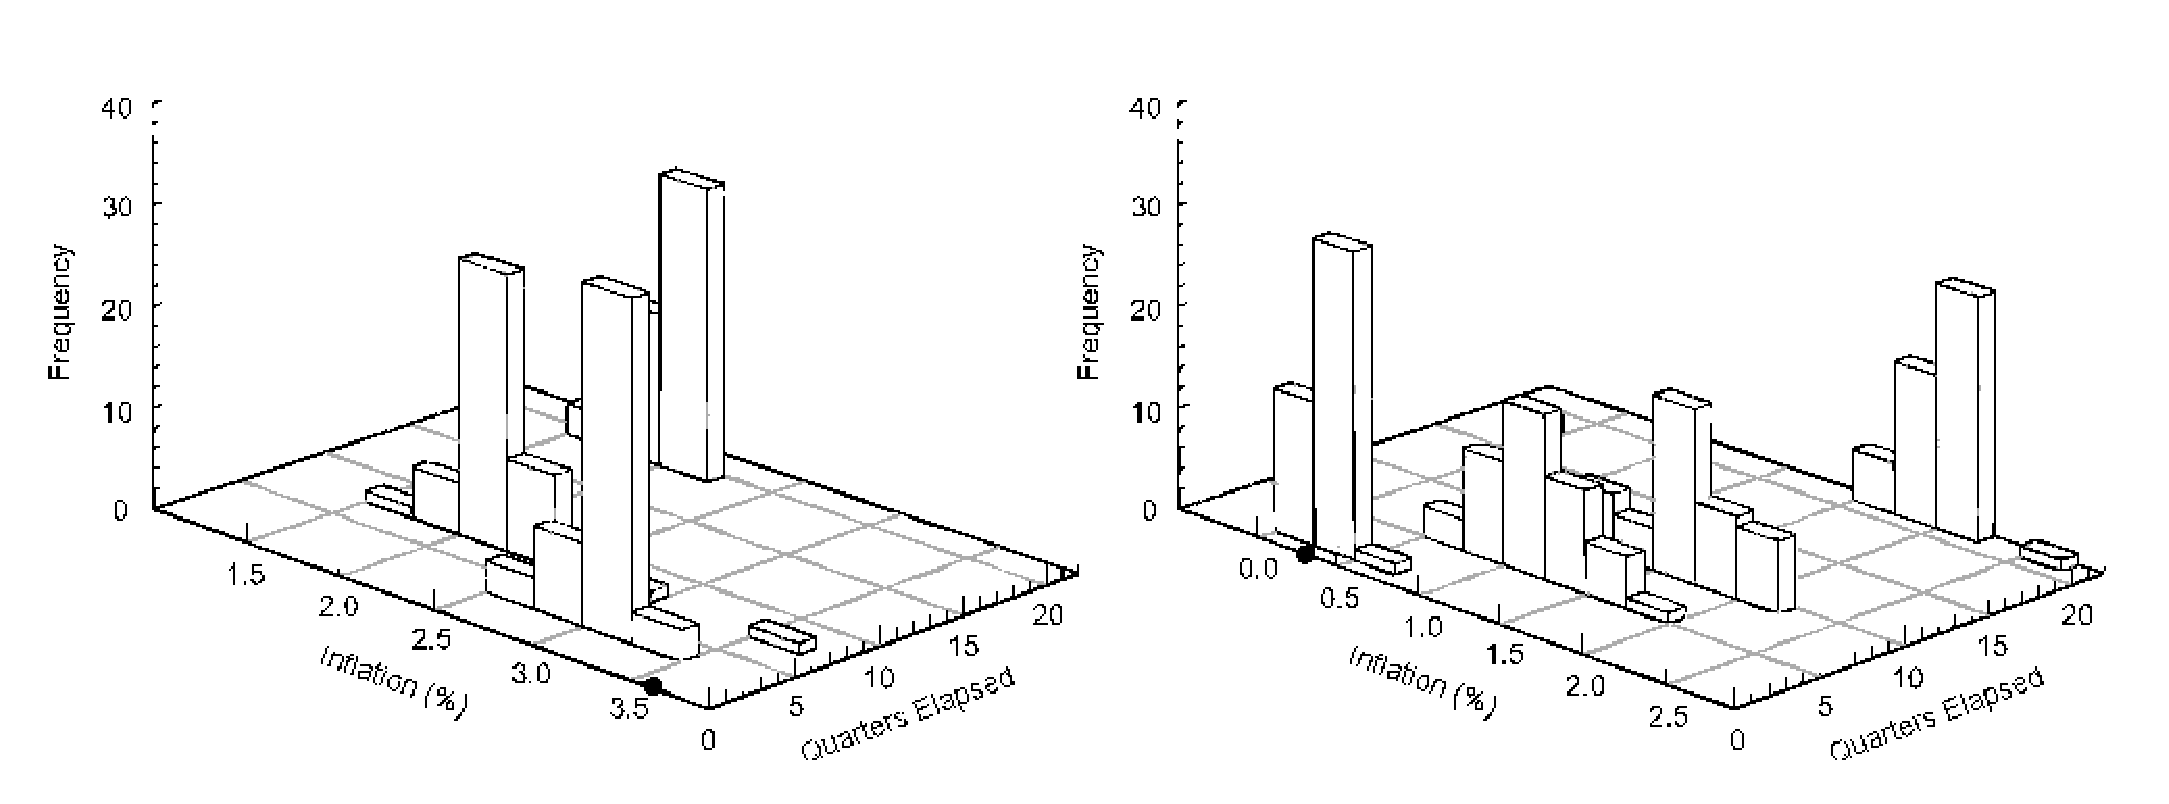
\includegraphics[width=1\columnwidth]{/Users/marshall/Documents/senior/thesis/figures/ecb_intuition_ed_tall_vector}

\caption{\label{fig:ecb_intuition}The marginal distribution of inflation forecasts
at the horizons included in the 2008Q2 (left) and 2009Q4 (right) SPFs.
The black dot indicates the inflation rate as of the month before
the SPF was administered.}
\end{figure}


The prices of many financial securities (inflation-indexed bonds,
for instance; see \citet[Eq. 2 in][]{woodward-1990}) depend on inflation
expectations over time. Given the vast array of inflation-linked securities
in the marketplace, the forecast horizons of the SPF may be too coarse
to be useful for practical purposes: for instance, we may be interested
in the distribution of inflation expectations halfway through a calendar
year. Thus emerges a natural arena in which we may ask questions of
inference and imputation given distributional data.

We formalize the problem as follows. Suppose we have an uncountable
sample space $\Omega$ of forecasters, each with her own model for
the evolution of HICP Euro Area inflation over time given current
inflation. We define the inflation expectation process $X=\{X_{t}\}$
where $X_{t}(\omega)$ is $\Omega\ni\omega$'s conditional expectation
for inflation at time horizon $t$ given current inflation. Furthermore,
we suppose $X$ evolves according to some model $\mathbb{P}$ that
is entirely unknown to us (the only constraint for this section that
we place on $\mathbb{P}$ is that it is absolutely continuous with
respect to the Gaussian measure). With this setup, the data provided
in any particular SPF are discrete observations of some finite number
of sample paths of $X$ under $\mathbb{P}$.

We are interested in what a particular SPF can tell us about the underlying
dynamics of the evolution of inflation expectations, and how we can
impute the distribution of $X$ at horizons not included in the SPF
questionnaire. The latter question can be intuitively understood as
asking what the forecasters would have said if we had surveyed them
for their inflation expectations at an arbitrary horizon. In the following
section, we will work with the $M=68$ SPFs conducted by the ECB from
1999Q1 through 2015Q4, obtained at \citep{spf-site}. \tabref{summary}
provides some summary statistics of this dataset.

\begin{table}
\centering \begin{tabular}{@{}lllll@{}} \toprule                                     & Mean  & SD   & Min.  & Max. \\ \midrule Forecasters surveyed                & 103.5 & 7.6  & 94    & 116  \\ Forecasters with complete responses & 44.3  & 6.1  & 33    & 62   \\ Inflation at time of SPF (\%)       & 1.76  & 0.90 & -0.70 & 4.10 \\ SD of nearest horizon forecasts (\%)     & 0.15  & 0.05 & 0.05  & 0.33 \\ SD of farthest horizon forecasts (\%)    & 0.21  & 0.07 & 0.09  & 0.55 \\ \bottomrule \end{tabular}

\begin{centering}
\begin{tabular}{lllll>{\raggedright}m{2cm}}
\multirow{1}{*}{} & \multirow{1}{*}{} &  &  &  & \tabularnewline
\end{tabular}
\par\end{centering}

\caption{\label{tab:summary}Summary statistics for the $68$ ECB SPFs administered
from 1999Q1 through 2015Q4.}
\end{table}



\section{Simple Inference on Inflation Expectations}

In this brief section, we verify that the proposed MCEM algorithm
consistently estimates the MKLDE in an empirical setting. In particular,
we posit a probability model $\mathbb{Q}_{\theta}$ under which $X$
is an OU diffusion governed by $\theta=(\mu,\lambda,\sigma)$. This
is an economically sensible model, consistent with the mean reversion
implicit in ECB's inflation targeting policy of aiming for ``inflation
rates of below, but close to, 2\% in the medium term'' \citep{targeting}.
Moreover, this is a mathematically convenient specification since
the transition density of the OU diffusion is analytically tractable.
We consider a particular SPF questionnaire, and let $\mathcal{T}=\{t_{1},\dots,t_{n}\}$
where $t_{1}>0$ be the set of horizons measured in quarters included
in the SPF and $\mathcal{O}\subseteq\Omega$ be the set of forecasters
with complete responses. Then, the average log-likelihood of the data
under $\mathbb{Q}_{\theta}$ is
\[
\bar{\ell}(\theta)=\frac{1}{|\mathcal{O}|}\sum_{\omega\in\mathcal{O}}\sum_{i=1}^{n}\mathcal{N}(X_{t_{i}}(\omega);\mu+(X_{t_{i-1}}(\omega)-\mu)e^{-\lambda t},\sigma^{2}(1-e^{-2\lambda t})/2\lambda),
\]
where $\mathcal{N}(x;\mu,\sigma^{2})$ is the Gaussian density with
mean $\mu$ and variance $\sigma^{2}$ and $X_{t_{i}}(\omega)$ is
forecaster $\omega$'s expectation of inflation at horizon $t_{i}$.
We set $X_{t_{0}}$ to the annualized HICP Euro Area inflation reported
at the end of the most recent month before the quarter that the SPF
was distributed (the SPF is usually distributed in the first month
of each quarter, so we can assume forecasters are conditioning on
the inflation print of the previous month). 

\begin{table}[b]
 \centering \begin{tabular}{@{}cccccl@{}} \toprule                         & Mean of $\theta^*$ & Bias (MCEM Est.)  &  \multicolumn{3}{l}{Cov. of bias ($\times 10^{-2}$)} \\ \midrule $\mu$             & 1.94 & -0.02\:            & \:1.23\:            &                &                \\ $\lambda$         & 0.23 & \;0.06\:           & -0.51\:           & 1.10           &                \\ $\sigma$          & 0.17 & \;0.00\:           & -0.56\:           & 0.50           & 0.24           \\ \bottomrule \end{tabular}


\begin{centering}
\begin{tabular}{lllll>{\raggedright}m{2cm}}
\multirow{1}{*}{} & \multirow{1}{*}{} &  &  &  & \tabularnewline
\end{tabular}
\par\end{centering}

\caption{\label{tab:mle-vs-mcem}Mean of the $\theta^{*}=\arg\max\bar{\ell}(\theta)$,
as well as the bias of MKLDE estimates, obtained by approximate MCEM,
relative to $\theta^{*}$, over $68$ ECB SPFs.}
\end{table}


By the comments in \chapref{EM}, $\arg\max\bar{\ell}(\theta)$, which
can be easily found through numerical optimization procedures, is
the parameter that asymptotically minimizes the K-L divergence of
the law of $X_{\mathcal{T}}$ under $\mathbb{Q}_{\theta}$ from its
law under $\mathbb{P}$. \tabref{mle-vs-mcem} reports the mean $\arg\max\bar{\ell}(\theta)$
and bias of the MKLDEs obtained through MCEM on the SPFs in our dataset,
measuring time in quarterly units. We note that the MKLDEs for $\mu$
and $\sigma$ obtained by approximate MCEM are effectively indistinguishable
from those obtained via direct maximization of the analytic likelihood.
Moreover, the MKLDE for $\mu$ aligns closely with intuition: On average,
forecasters seem to expect the reversion of inflation to the medium-term
inflation target of the ECB (below, but close to, $2\%$).

On the other hand, the bias is non-trivially positive for the MKLDE
of $\lambda$, suggesting that the thin-tailedness of the approximate
bridges can in fact affect the quality of approximate MCEM estimates
in empirical situations. The computational cost of exact MCEM, however,
can still be high enough that the practitioner will need to weigh
the utility of slightly more accurate estimates against significantly
longer running times on a case-by-case basis.


\section{Putting It All Together}

In the final original section of this thesis, we synthesize the methods
developed here by answering the following question: What can we say,
given a finite number of sample paths of $X$ observed at discrete
time points, about the distribution of $X$ at arbitrary horizons,
when the parameters governing $X$ are unknown? In particular, we
propose a generalized bridge-based imputation scheme given distributional
data and a stochastic model known only up to its parameters. We show
such a scheme reduces mean out-of-sample estimated K-L divergence
of interpolations from the truth vis-�-vis a baseline linear interpolation
for the ECB SPF dataset, using models with tractable and intractable
log-likelihood. 

To begin, we consider a particular SPF containing forecasts from a
finite set of forecasters at every time $t\in\mathcal{T}=\{t_{1},\dots,t_{n}\}$
where $t_{1}>0$. Let $\hat{\nu}$ be the $(n+1)$-dimensional empirical
distribution induced by these forecasts and the fixed inflation print
at $t_{0}=0$, the month before the SPF was administered (noting that
the dependence structure of this distribution is given by the indexing
of forecasts at different horizons to particular forecasters). Recall
that the forecasts contained in the SPF can be understood as samples
from $X_{\mathcal{T}}$ under the true but unknown model $\mathbb{P}$,
and let $\mathbb{P}_{X_{\mathcal{T}}}$ be the law of $X_{\mathcal{T}}$
under $\mathbb{P}$. 

\begin{figure}
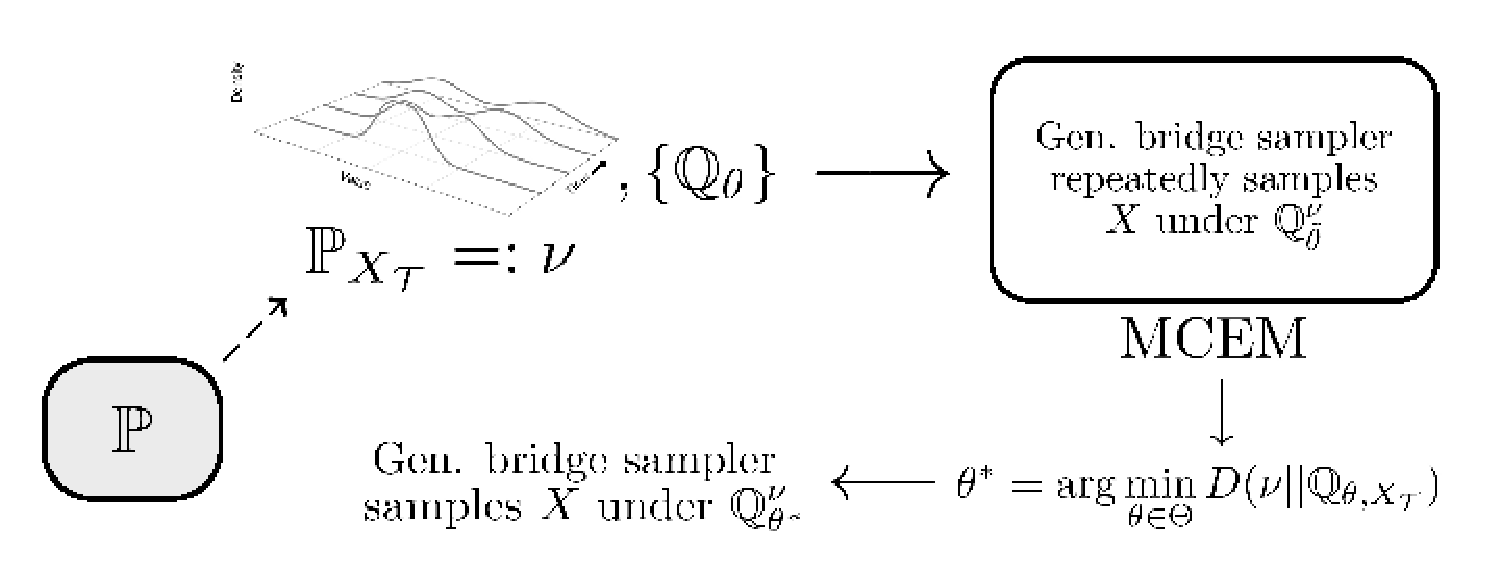
\includegraphics[width=1\columnwidth]{/Users/marshall/Documents/senior/thesis/figures/imputation_scheme}

\caption{\label{fig:imputation}A schematic depiction of the proposed imputation
method, in which the MCEM algorithm for estimating the MKLDE and the
generalized bridge samplers developed in previous chapters are used
to approximate the law of $X$ under $\mathbb{P}$ with samples from
$X$ under $\mathbb{Q}_{\theta^{*}}^{\nu}$. $\mathbb{P}$ is enclosed
in a grey box, highlighting that we do not have access to $\mathbb{P}$
but rather only the law of $X_{\mathcal{T}}$ under $\mathbb{P}$.}
\end{figure}


Now, fix a parameterized family of models $\{\mathbb{Q}_{\theta}\}$.
Suppose we have the parameter $\theta^{*}$ that minimizes the K-L
divergence of the distribution of $X_{\mathcal{T}}$ under $\mathbb{Q}_{\theta}$
from its true distribution $\mathbb{P}_{X_{\mathcal{T}}}$. We posit
that a reasonable guess for the law of $X$ under $\mathbb{P}$ when
only given $\mathbb{P}_{X_{\mathcal{T}}}$ is the law of $X$ under
the $(X_{\mathcal{T}},\mathbb{P}_{X_{\mathcal{T}}})$-conditioning
of $\mathbb{Q}_{\theta^{*}}$.\footnote{A theoretical justification of this statement is a pressing direction
for future research.} It follows that a natural imputation method for the distribution
of $X$ under $\mathbb{P}$ at arbitrary horizons, schematized in
\figref{imputation}, is to first estimate the MKLDE $\theta^{*}$,
then simulate $\mathbb{P}_{X_{\mathcal{T}}}$-bridges of $X$ under
$\mathbb{Q}_{\theta^{*}}$; here, we use $\hat{\nu}$ as a plug-in
estimate for $\mathbb{P}_{X_{\mathcal{T}}}$. \figref{imputation}
highlights how the questions of inference and imputation on distributional
data, and by extension the MCEM algorithm and the generalized bridge
samplers developed in \chapref{EM} and \chapref{4}, are intimately
related.

We cross-validate the proposed imputation method as follows, setting
\begin{aenumerate}
\item $\hat{\nu}_{t_{i}}$ to be the empirical distribution induced by the
forecasts at $t_{i}$,
\item $\hat{\nu}_{-t_{i}}$ to be the the $n$-dimensional empirical distribution
of the forecasts at all horizons except $t_{i}$, and
\item $X_{-t_{i}}\coloneqq X_{\mathcal{T}\setminus t_{i}}$.
\end{aenumerate}
\begin{figure}
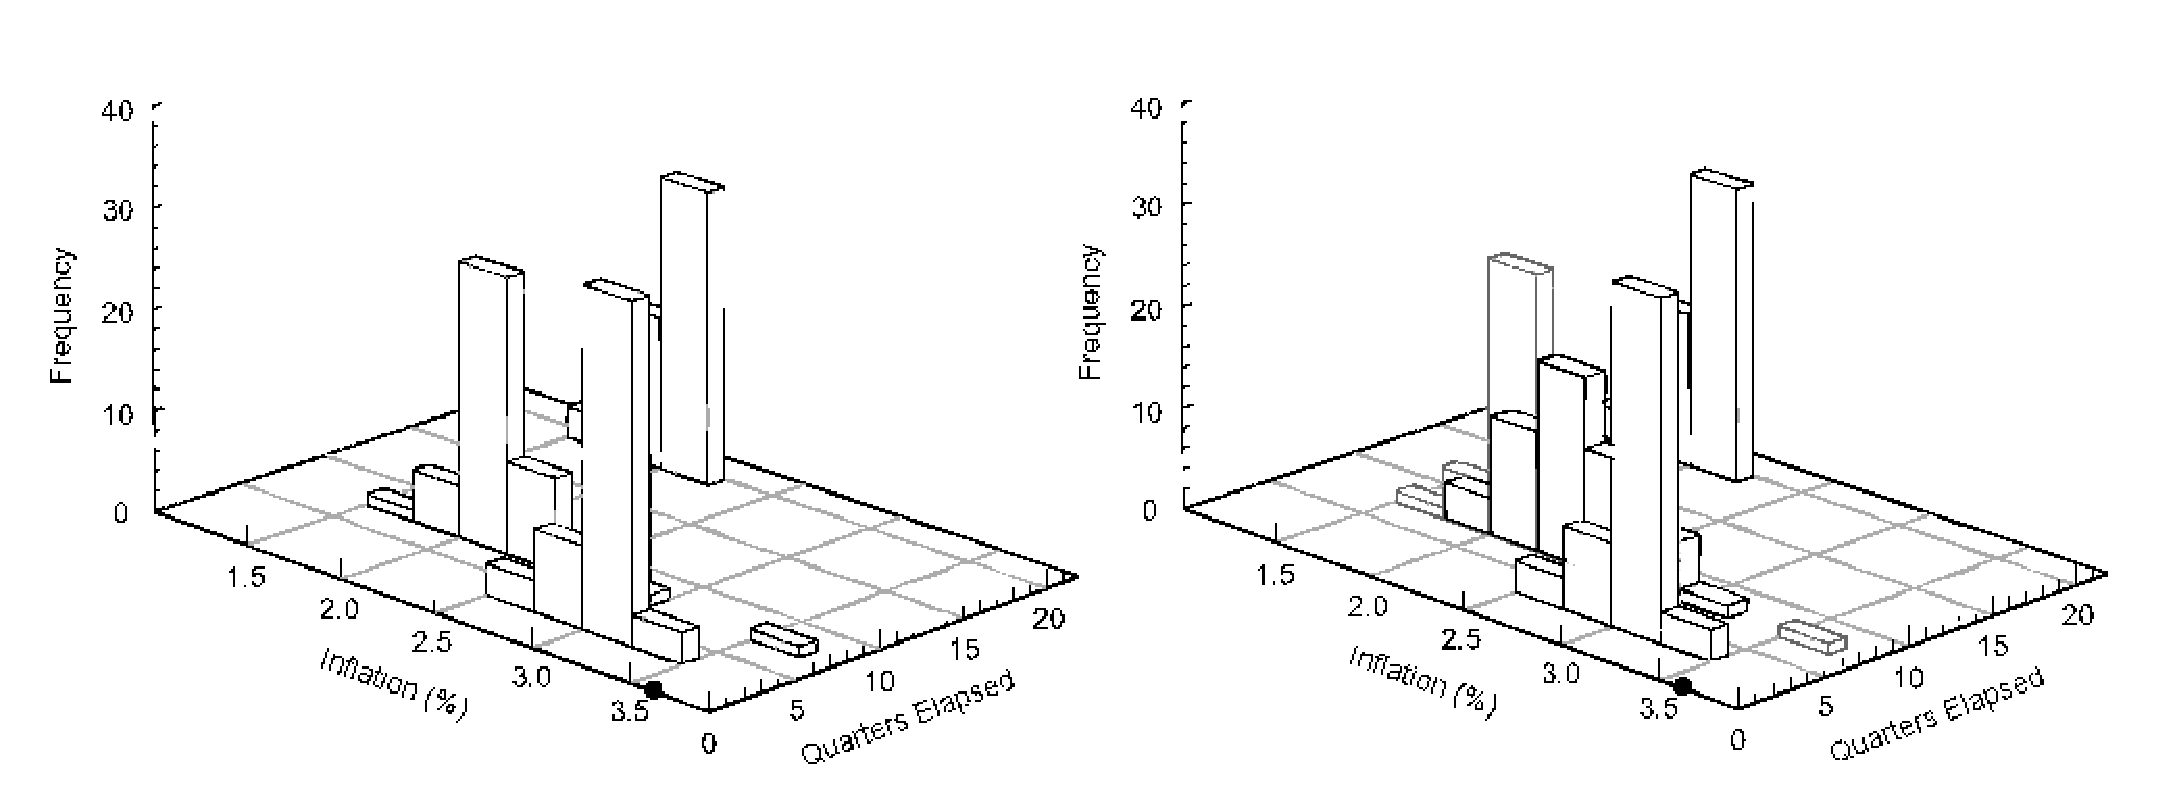
\includegraphics[width=1\columnwidth]{/Users/marshall/Documents/senior/thesis/figures/cross_v_intuition}

\caption{\label{fig:cv}A visualization of the cross-validation method for
assessing imputation strategy performance. The left graphic depicts
data from a particular SPF. The right graphic depicts an imputed distribution,
in black, superimposed on the original true distribution, to be used
to validate the imputated distribution, in gray.}
\end{figure}


First, we estimate the MKLDE $\theta_{-t_{i}}^{*}$ for $X$ under
$\mathbb{Q}_{\theta}$ given $\hat{\nu}_{-t_{i}}$ using approximate
MCEM. Then, we draw samples of $X_{t_{i}}$ under the Baudoin-$(X_{-t_{i}},\hat{\nu}_{-t_{i}})$
conditioning of $\mathbb{Q}_{\theta_{-t_{i}}^{*}}$ to induce an empirical
imputed distribution $\tilde{\nu}_{t_{i}}$. Finally, we use $\tilde{\nu}_{t_{i}}$
and $\hat{\nu}_{t_{i}}$ to consistently estimate the out-of-sample
Kullback-Liebler divergence of the law of $X_{t_{i}}$ under the Baudoin-$(X_{-t_{i}},\mathbb{P}_{X_{-t_{i}}})$
conditioning of $\mathbb{Q}_{\theta_{-t_{i}}^{*}}$ from its law under
$\mathbb{P}$ using the estimator of \citet[Theorem 1 in][]{perez-cruz-2008}.
Since forecasters often give the same forecasts for inflation at a
particular horizon, and the \citet{perez-cruz-2008} estimator requires
an empirical distribution function induced by unique samples, we add
arbitrarily small normally distributed noise $(\sigma^{2}\approx10^{-4})$
to the forecasts that induce $\hat{\nu}_{t_{i}}$. Furthermore, since
$n\geq3$ for all SPFs in our dataset, we consider $i\in\{1,2\}$.
\figref{cv} intuitively visualizes the cross-validation process:
The left side depicts the original SPF dataset, while the right side
depicts the removal of the marginal distribution at $t_{2}=8$ and
a new imputed marginal distribution at that time. The K-L divergence
of the imputed distribution from the grayed-out marginal distribution
is estimated as described.

To put the performance of our proposed imputation scheme into context,
we set a linear interpolation scheme as our baseline. In particular,
a linear interpolation $\tilde{X}_{t}$ of the forecasts $\{X_{t_{i}}\}_{t_{i}\in\mathcal{T}}$
of a particular forecaster is the function 
\begin{equation}
\tilde{X}_{t}=\frac{(t_{i}-t)X_{t_{i-1}}+(t-t_{i-1})X_{t_{i}}}{t_{i}-t_{i-1}}\label{eq:lininterp}
\end{equation}
for $t_{i-1}\leq t\leq t_{i}$ and $i=2,\dots,n$. This scheme is
not simply a straw man; its non-parametric nature makes it an extremely
robust imputation method, and it is simple to implement. Therefore,
in order for a complex scheme like the one proposed in this chapter
to be seen as a viable alternative for imputation, it must offer meaningful
improvements over linear interpolation. 

Our prior belief is that our scheme should in fact improve substantially
on linear interpolation. For instance, inflation expectations are
likely state-dependent: Central banks are wary of overshooting their
inflation targets, and thus can be expected to deploy monetary policy
to slow the velocity of inflation movements as inflation approaches
their target. A linear interpolation will not capture this expected
deceleration in inflation expectations while various It� diffusions,
including the OU diffusion, may be able to.

Though the case of an OU model was useful in the previous section
as an illustrative example, the development of an MCEM algorithm was
motivated by the fact that there are a wide range of diffusions for
which transition densities are not analytically available. As such,
in addition to a model $\mathbb{Q}_{\theta}^{OU}$ under which $X$
is an OU diffusion, we consider a model $\mathbb{Q}_{\theta}^{HYP}$
under which $X$ evolves according to 
\begin{equation}
dX_{t}=\frac{-\lambda(X_{t}-\mu)dt}{\sqrt{\delta^{2}+(X_{t}-\mu)^{2}}}+\sigma dW_{t},\label{eq:hypdiff}
\end{equation}
i.e. a model under which $X$ is a hyperbolic diffusion. This type
of diffusion was first proposed by \citet[Eq. 6.2 in][]{barndorff-1978},
who noted such a diffusion has stationary distribution 
\[
f(x)=\frac{e^{-\frac{2\lambda}{\sigma^{2}}\sqrt{\delta^{2}+(x-\mu)^{2}}}}{2\delta K_{1}(2\delta\lambda/\sigma^{2})},
\]
where $K_{1}$ is a modified Bessel function of the third kind with
index $1$. Hyperbolic diffusions are It� diffusions with finite speed
measure, and thus satisfy the assumptions made in \chapref{2}; however,
they do not admit a tractable transition density. We can see by inspection
of (\ref{eq:hypdiff}) that this model incorporates linear mean reverting
drift dynamics, similar to those of an OU process, when $|X_{t}-\mu|$
is small, and constant mean reverting drift when $|X_{t}-\mu|$ is
large. Since the hyperbolic diffusion, like the OU process, has constant
diffusion coefficient, its Lamperti transform and the requisite functions
for performing MCEM are easy to find.

\tabref{wilcoxon} presents the mean and median estimated K-L divergences
of the imputed distributions at $t_{1}$ and $t_{2}$ from the true
distributions over each SPF in the data set, using the generalized
bridge-based imputation scheme and the linear interpolation method
outlined in (\ref{eq:lininterp}). In all SPFs considered, $t_{1}$
and $t_{2}$ are time horizons between $1-4$ and $5-8$ quarters
respectively. 

\begin{table}[t]

\centering \begin{tabular}{@{}lccccm{0.1em}cc@{}} \toprule \multirow{2}{*}{Horizon \& Imputation Scheme} & \multirow{2}{*}{Mean} & \multirow{2}{*}{Median} & \multicolumn{2}{c}{Wilc. $p$ vs.}  & & \multicolumn{2}{c}{Sign $p$ vs.} \\ \cmidrule(l){4-5} \cmidrule(l){7-8}                                                             &         &                 & LI   & OU  & & LI   & OU                 \\ \midrule \emph{1-4 Quarter Horizon}                                  &         &                 &      &     & &      &                 \\ \:\:\:\:Linear Interpolation (LI)                           & 1.43    & 1.29            &      &     & &      &                    \\ \:\:\:\:Gen. Bridge (OU)                                    & 1.14    & 0.95            & 0.01 &     & & 0.08 &                    \\ \:\:\:\:Gen. Bridge (Hyp.)                                  & 1.18    & 0.96            & 0.00 & 0.61& & 0.14 & 0.85                  \\ \emph{5-8 Quarter Horizon}                                  &         &                 &      &     & &      &                 \\ \:\:\:\:Linear Interpolation (LI)                           & 0.96    & 0.81            &      &     & &      &                \\ \:\:\:\:Gen. Bridge (OU)                                    & 0.70    & 0.78            & 0.04 &     & & 0.23 &                  \\ \:\:\:\:Gen. Bridge (Hyp.)                                  & 0.74    & 0.61            & 0.01 & 0.15& & 0.09 & 0.32                \\
\bottomrule \end{tabular}


\begin{centering}
\begin{tabular}{lllll>{\raggedright}m{2cm}}
\multirow{1}{*}{} & \multirow{1}{*}{} &  &  &  & \tabularnewline
\end{tabular}
\par\end{centering}

\caption{\label{tab:wilcoxon}Mean and median out-of-sample estimated K-L divergences
of imputed inflation expectations from the distribution of $X$ under
$\mathbb{P}$ for various horizons and imputation schemes, across
$52$ SPFs (any SPFs for which approximate MCEM did not converge were
dropped). K-L divergences were estimated using the \citet{perez-cruz-2008}
estimator. If $X$ and $Y$ are the true K-L divergences under the
row and column imputation schemes, Wilcoxon $p$-values (Wilcox. $p$)
and sign $p$-values (Sign $p$) are obtained from the Wilcoxon signed-rank
test and the sign test respectively, under the alternative hypothesis
that $P(X-Y<0)>1/2$.}
\end{table}


\tabref{wilcoxon} also presents $p$-values from tests on the paired
differences of the K-L divergences between the various imputation
schemes; these can be used to evaluate the statistical significance
of the reductions in K-L divergence offered by a particular imputation
scheme over another. Exploratory data analysis suggests that the paired
differences of K-L divergences deviate substantially from normality;
\tabref{wilcoxon} therefore presents the $p$-values from a Wilcoxon
signed-rank test for whether the paired differences are centered at
zero. However, these paired differences also display some amount of
skew. Given the relatively small sample size ($52$ paired differences),
it is not clear whether this skewness suggests a material violation
of the symmetry assumption underlying the Wilcoxon signed-rank test;
as such, we also present $p$-values obtained from the sign test,
whose few assumptions can be confirmed to be satisfied by our data.

We see that the generalized bridge-based methods offer qualitatively
large reductions (on the order of $20-30\%$) in the mean and median
of out-of-sample estimated K-L divergences vis-�-vis a linear interpolation
scheme, at both horizons considered. The Wilcoxon signed-rank test
reveals that the improvements over the linear interpolation scheme
offered by our generalized bridge-based methods are statistically
significant at the $95\%$, and sometimes $99\%$, level. The sign
test, on the other hand, only begins to reveal significant differences
at the $90\%$ level; however, we ought to keep in mind that the sign
test is an extremely conservative test that discards any information
about the magnitude of the K-L divergence reductions. We believe that
the truth is somewhere between the Wilcoxon signed-rank $p$-values
and the sign test $p$-values: While there is some evidence that the
true paired difference distribution may be skewed, the sign test seems
to discard too much information to convincingly capture a statistically
significant difference in the quality of our imputation schemes. Having
examined the evidence, we update to a fairly strong belief that bridge-based
imputation does in fact offer better imputations of inflation expectations
than linear interpolation, taking into account
\begin{aenumerate}
\item the qualitatively large reduction in K-L divergence under a generalized
bridge-based imputation scheme,
\item the array of relatively small $p$-values even from low power tests
like the sign test, and
\item our prior that linear evolution should not fully capture the complex
dynamics of inflation expectations.
\end{aenumerate}
We do not qualitatively or formally detect any meaningful difference
between bridge-based imputation under a hyperbolic or OU diffusion.
This is not unexpected; the parameter estimates for the hyperbolic
diffusion result in an implied stationary distribution only slightly
fatter-tailed than the stationary OU distribution. Moreover, if the
ECB faithful to its inflation target, inflation should not be deviating
from $2\%$ substantially, and so the differences in mean reversion
dynamics between the two processes when they are far from their mean
should emerge infrequently.

Though the reduction in K-L divergence is non-trivial and statistically
significant when using bridge-based imputation over linear interpolation,
the magnitude of the K-L divergences remains large. For reference,
the K-L divergence of a standard Gaussian distribution from an even
mixture of Gaussian distributions centered at $-3/2$ and $3/2$ with
unit variance is estimated to be in the neighborhood of $0.60$. This
is about the same as the lowest achieved estimated K-L divergence
from the truth in our experiments. The estimated K-L divergences here
therefore appear to suggest that conditional expectations of inflation
are not particularly well-modeled by the selected It� diffusions,
and even less so by a piecewise linear function. This is not entirely
surprising; for instance, there is no reason to think that conditional
inflation expectations should follow time-homogenous dynamics. Nevertheless,
the methodology proposed here can provide a useful first step modeling
the evolution of stochastic processes, conditional on their distribution
at discrete points in time. 

\begin{figure}
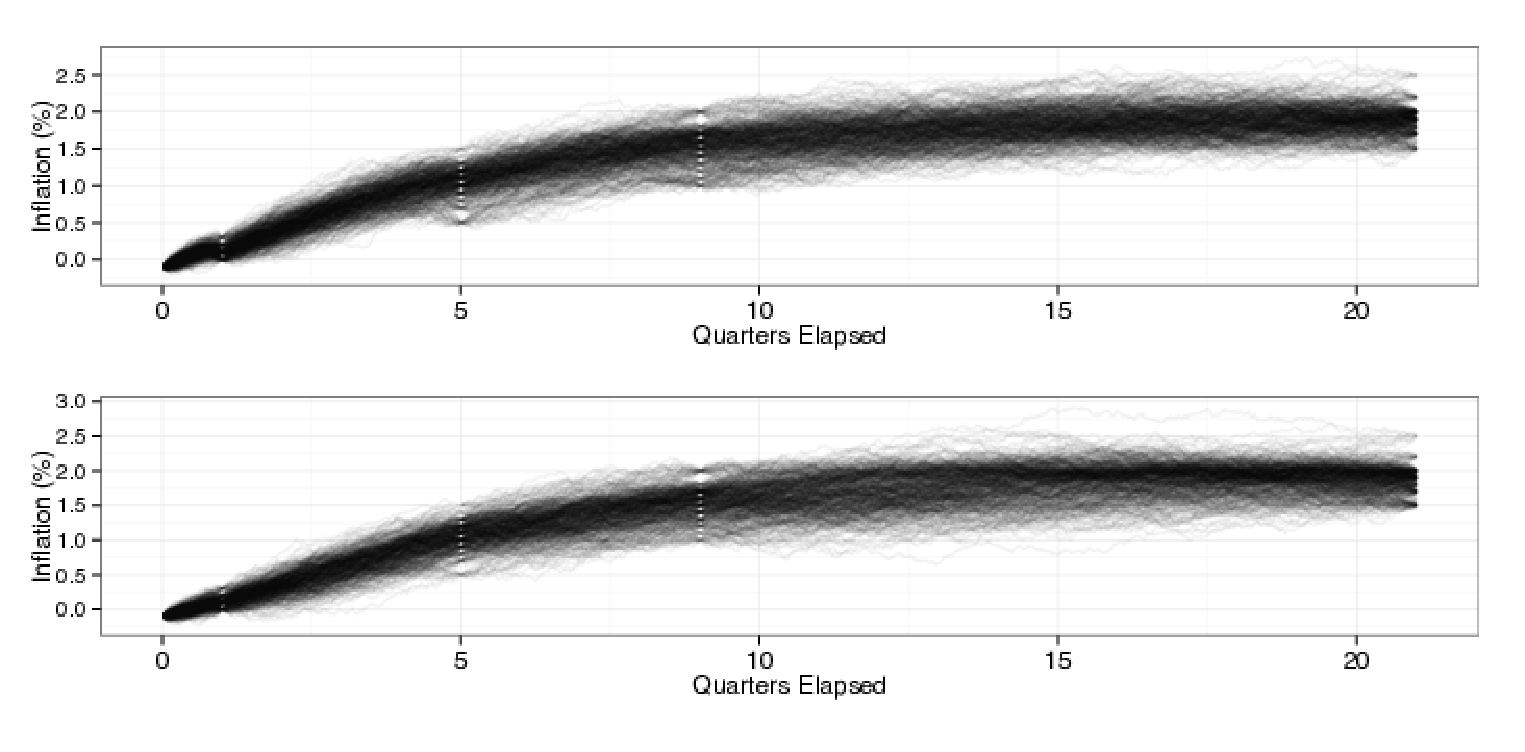
\includegraphics[width=1\columnwidth]{/Users/marshall/Documents/senior/thesis/figures/cont_path}

\caption{\label{fig:cont_path}500 sample paths of $\hat{\nu}$-bridges of
$X$ under $\mathbb{Q}_{\theta^{*}}^{OU}$ (top) and $\mathbb{Q}_{\theta^{*}}^{HYP}$
(bottom), where $\theta^{*}$ is the MKLDE of $\mathbb{Q}_{\theta}^{OU}$
and $\mathbb{Q}_{\theta}^{HYP}$ from $\mathbb{P}$ respectively,
using the 2015Q4 SPF.}
\end{figure}


We conclude this chapter with a visualization of the final product
of this thesis in \figref{cont_path}. Using an approximate MCEM scheme
to infer the MKLDE of $\mathbb{Q}_{\theta}^{OU}$ and $\mathbb{Q}_{\theta}^{HYP}$
given $\hat{\nu}$, we plot repeated samples of $\hat{\nu}$-bridges
of $X$ under $\mathbb{Q}_{\theta^{*}}^{OU}$ and $\mathbb{Q}_{\theta^{*}}^{HYP}$
for the most recently conducted SPF (2015Q4). This figure highlights
the differences in behavior of the two diffusions when far from the
mean. In particular, the shortcomings of the time-homogenous OU model's
linear mean reversion are laid bare: the imputed paths revert to the
inflation target far too quickly initially before being forced down
to the relatively low inflation expectations at the end of the 2015.
Time-inhomogeneity therefore appears to be an important feature of
inflation expectations as of 2015Q4, with expected inflation remaining
low in the short-term, and rapidly accelerating in the medium-term.
However, this is a problem of model selection and not of methodology;
as such, \figref{cont_path}, representing the synthesis of the methods
developed here to perform inference and imputation on the forecasts
of modern-day macroeconomic oracles, is a fitting conclusion to the
original portion of this thesis.



\chapter{Conclusions and Future Directions\label{chap:7}}

We conclude by briefly reviewing the contributions made and suggesting
future directions for research.

This thesis considers the novel (to the best of our knowledge) problem
of statistical inference when given the distribution, instead of particular
observations, of a stochastic process at discrete points in time.
This is a generalization of the classical problem of inference on
discrete observations that has been well-studied in the literature.
We develop novel inference strategies when given distributional data
and the first samplers for a particular class of generalized bridges.
Simulations and empirical studies demonstrate the correctness of the
methods described and their broad applicability.

Future directions for research abound, especially given the novel
problem of this thesis. We highlight some potential lines of exploration
here. Most pressingly, a formal investigation into the properties
of the imputation scheme proposed in \chapref{6} is needed to justify
its use. It seems intuitive that a model which minimizes its K-L divergence
from a true but unknown model, conditioned on the available distributional
data from the true model, is our best guess at the underlying truth;
however, no attempt is made in this thesis to formalize this thought.
Since we imagine most applications of the methods presented in this
paper will involve distributional data and a stochastic model specified
only up to its parameters, rigorously justifying the proposed imputation
scheme is of utmost importance.

Of equal urgency is a rigorous characterization of the properties
of the MKLDE. This would complement the mathematical remarks made
in \chapref{EM} and set the results of this thesis on firmer theoretical
ground. Such characterizations ought to come fairly easily from existing
results, given the close links between MKLDE and MLE.

A third avenue of research comes from the simulation results presented
in \chapref{5}, showing that the generalized bridge samplers appeared
to be empirically robust against the relaxation of a variety of assumptions
in their derivation. We conjecture based on simulations for Wiener
bridges that in particular, the restriction of diffusions to those
with finite speed measure considered in this thesis is overly strict.
Perhaps a sampler (potentially more ``approximate'', in some sense,
than the sampler proposed here) for more general diffusions is not
too far from reach.

Empirically, an area ripe for an application of the methods proposed
in this thesis is the modeling of asset prices based on distributional
data from options markets: Having access to the market-determined
distribution of prices at arbitrary horizons would be incredibly valuable
for practitioners and academics alike. Notwithstanding the trading
strategies that could immediately result, evaluating the efficiency
of options markets in pricing the distributional features of asset
prices over time would be a particular area of academic interest.


\cleardoublepage{}\include{Bibliography}%
\begin{comment}

\part{Appendix}

\include{Chapter0A}

\cleardoublepage{}

\cleardoublepage{}

\include{Colophon}

\cleardoublepage{}

\include{Declaration}
\end{comment}

\end{document}
